\documentclass{llncs}

\usepackage{subfigure}
\usepackage{color}
\usepackage[usenames,dvipsnames]{xcolor}
\usepackage{graphicx}
\usepackage[numbers, sectionbib]{natbib}
\usepackage{tabularx}
%\usepackage{float}
\usepackage{afterpage}

\usepackage{anyfontsize}
\usepackage{fontspec}
\setmainfont{Times New Roman}

\usepackage{dblfloatfix}
\setlength{\textfloatsep}{4pt plus 1.0pt minus 1.0pt}
\setlength{\floatsep}{4pt plus 1.0pt minus 1.0pt}
\setlength{\intextsep}{4pt plus 1.0pt minus 1.0pt}

\setlength{\dbltextfloatsep}{4pt plus 1.0pt minus 1.0pt}
\setlength{\dblfloatsep}{4pt plus 1.0pt minus 1.0pt}


\usepackage{listings}
\lstnewenvironment{code}[1][]%
  {\minipage{0.9\linewidth} 
   \lstset{basicstyle=\ttfamily\footnotesize,frame=single,#1}}
  {\endminipage}

\definecolor{lightgray}{gray}{0.95}

\begin{document}

\title{Evaluating Open Information Extraction for Ontologization of a Thematic Domain}

\author{Gopala Krishna Koduri\inst{1} \and Siva Reddy\inst{2} \and Bharat Ram Ambati\inst{2} \and Xavier Serra\inst{1}}
\institute{Music Technology Group, Universitat Pompeu Fabra, Barcelona, Spain \and
Institute for Language, Cognition and Computation, University of Edinburgh, UK \\
\email{gopala.koduri@upf.edu}
}

\maketitle

\begin{abstract}
In the past decade, domain-independent approaches to information extraction have paved way for its web-scale applications. Adapting them further to acquire knowledge from thematic domains can greatly reduce the need for manual knowledge engineering. This requires understanding how amenable the assertions extracted by such approaches are to ontologization. To this extent, we propose a framework for a comparative extrinsic evaluation of the open information extraction systems. The first part of the framework compares the volume of assertions along different dimensions with an aim to understand their coverage of the domain quantitatively. In the second part, the assertions are evaluated qualitatively by employing them in three of the fundamental tasks of ontologization: entity identification, concept identification and semantic relation extraction. The framework is demonstrated using the Indian art music domain. The combined observations are shown to be useful in gathering insights about not only the quality of the assertions, but also the nature of the approaches.
\end{abstract}

\section{Introduction}
\label{sec:intro}
The advent of the semantic web and the linked open data movements have not only resulted in a growing number of community-built structured data sources, but also catalyzed the development of domain-independent approaches for extracting information from unstructured text, further enriching them. Open information extraction (OIE) is one such paradigm that has emerged in the past decade, and has been used to extract assertions from unstructured data at web-scale with a considerable success~\cite{Etzioni2008a}. Until recently, domain-specific approaches to information extraction from text required manual knowledge engineering as a prerequisite~\cite{Sarawagi2008}. The OIE approaches, however, do not require a prespecified vocabulary and/or relation-specific input. Therefore, adapting them to information extraction from thematic domains would alleviate the need or manual knowledge engineering.

The process of channeling the assertions extracted from these approaches into a coherent knowledge-base itself poses certain challenges. There has been little work so far to identify and address such issues. The advances in OIE, including the recent systems such as NELL\footnote{http://rtw.ml.cmu.edu/rtw/}, are largely directed towards taking advantage of the volume of web data. In doing so, the recall of the systems is often traded off for a good precision. The adaptation of such systems to acquire knowledge from a given domain is an exciting prospective direction. Soderland \textit{et.al}~\cite{Soderland2010} have first attempted to adapt TextRunner system~\cite{Etzioni2008a} to populate the knowledge-base concerning facts in the football game domain. One of their findings is that the limited recall of the OIE systems is the major bottleneck in acquiring a good coverage of the relation types.

In this paper, we propose a comprehensive framework for a comparative evaluation of the open information extraction approaches for ontologization of a thematic domain. The first part of the framework compares the volume of extracted assertions along different aspects of a given domain with an aim to understand the coverage of the domain quantitatively. In the second part of the framework, the assertions are used in three fundamental tasks of ontologization: entity identification, concept identification, and semantic relation extraction. The framework is demonstrated using Indian art music domain, and the results from each task are validated against structured content in Wikipedia and/or are manually checked as necessary. The results from the two parts of the framework, when juxtaposed against each other, give us concrete insights into the differences between the performances and the nature of the approaches.

The remainder of the paper is organized as follows. In sec.~\ref{sec:oie}, the OIE approaches that we chose to compare are discussed and in sec.~\ref{sec:data},  an overview of the data we work with is presented. In sec.~\ref{sec:framework}, we present the framework with various quantitative and qualitative measures for analyzing the quality of assertions extracted, and in sec.~\ref{sec:results}, we demonstrate it on the music domain. Sec.~\ref{sec:conclusions} concludes the paper with our remarks and future direction of this work.

\section{Open Information Extraction}
\label{sec:oie}
Information extraction is the task of obtaining a set of assertions from the natural language text, featuring the entities and the relations of the corresponding domain. The approaches are diverse ranging from those which learn from the labeled training samples for the desired set of target relations, to those which operate in an unsupervised manner. An easy access to large volume of unstructured text on the web has necessitated approaches that scale appropriately to take advantage of this data. Open information extraction aims to extract the assertions from voluminous data without requiring a pre-specified vocabulary or labeled data for relations~\cite{Etzioni2008a}.

\subsection{ReVerb \& OpenIE 4.0}
For demonstrating our evaluation framework, we choose two state-of-the-art OIE systems: ReVerb~\cite{Fader2011a} and OpenIE 4.0~\cite{Mausam2012a}, which are shown to have outperformed the earlier systems such as TextRunner~\cite{Etzioni2008a}, $woe^{pos}$ and $woe^{parse}$~\cite{Wu2010a}. ReVerb addresses the issue of incoherent and uninformative extractions\footnote{We have used the terms \textit{assertions} and \textit{extractions} analogously.} found with the former systems, by using few syntactic and lexical constraints. OLLIE~\cite{Mausam2012a} is a successor of ReVerb, and includes the noun-mediated relations which are not handled by the latter. It also incorporates the context of the assertions in the form n-ary relations. OpenIE 4.0 employs a similar methodology to that of OLLIE, to retrieve assertions using semantic role labeling, also known as shallow semantic parsing. The implementations for both ReVerb and OpenIE 4.0 are available online\footnote{Available at https://github.com/knowitall/}.

\subsection{Semantic parsing}
On the other hand, deep semantic parsing is an active research topic in the natural language processing (NLP) community, which aims to obtain a complete logical form of a given sentence. It is used in applications such as question-answering systems, robotic navigation and further has several direct implications for OIE as it is domain-independent and is shown to be web-scalable~\cite{Harrington2007}. To our knowledge, there is no existing literature that compares semantic parsing with the likes of ReVerb and OpenIE 4.0. We therefore built an information extraction wrapper around a state-of-the-art semantic parser and compare with the selected OIE systems. What follows is a brief description of this system.

We use Combinatory Categorial Grammar (CCG)~\cite{Steedman:2000:SP:332037} as our grammatical framework to parse natural language sentences to logical representation. CCG is known for its transparency between syntax and semantics, i.e. given the syntactic structure (CCG derivation) of a sentence, a semantic representation can be built deterministically from its derivation. Each word in a sentence is first assigned a CCG category based on its context. Each category represents the syntactic constraints that the word has to satisfy. For example, in Fig.~\ref{fig:ccg_sample}, the word \textit{plays} is assigned a syntactic category $(S\backslash NP)/NP$ implying that \textit{plays} take a noun ($NP$) argument on its right, and a noun argument ($NP$) on its left to form a sentence ($S$). An equivalent semantic category in terms of a lambda function is constructed from the syntactic category, here $\lambda x. \lambda y. \mathrm{plays}(subj,~y) \wedge \mathrm{plays}(obj,~x)$ with \textit{plays} representing the predicate, $x$ and $y$ representing the object (guitar) and subject (John) arguments. CCG defines a set of combinators using which the adjacent categories combine to form syntactic categories of larger text units like phrases (\textit{e.g:} plays guitar), from there on leading to parsing a whole sentence. Correspondingly, the lambda functions of the categories compose, eventually leading to the semantic representation of the sentence. The advantage with CCG is that the complexity of obtaining a logical representation of a sentence is simplified into the task of assigning categories to words. We use a modified version of Boxer~\cite{Bos2004} to further convert our sentences of interest to the triple form (subject, relation phrase, object).
\begin{figure}[!t]
\centering
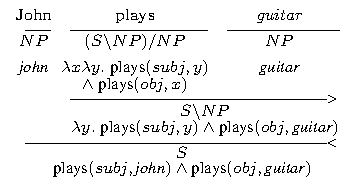
\includegraphics[width=0.6\linewidth]{figures/ccg_sample.pdf}
\caption{An example showing the CCG syntactic and semantic derivation of `John plays guitar'.}
\label{fig:ccg_sample}
\end{figure}

\section{Data}
\label{sec:data}
A major challenge in developing technologies for the exploration and the navigation of music repertoires from around the world lies in obtaining and using their cultural context. The vocabulary used for describing and relating the entities (musical concepts, roles of people involved etc) differs to a great extent from music to music. Most commercial platforms have a limited view of such context, resulting in poor navigation and exploration systems that fail to address the cultural diversity of the world.  Within the music information research community, there is a growing interest for developing culture-aware approaches to address this problem~\cite{Serra2011}. Such approaches are diverse in terms of the data they work with (audio, metadata and contextual-data) and methodologies they employ~\cite{Serra2013a}. 

However, to our knowledge, there are no major attempts that use web text, arguably the largest openly available data source. As a first step in this direction, we choose to demonstrate our framework in the music domain. Indian art music traditions: Carnatic and Hindustani, have a very distinct character, especially when compared to the popular music styles that drive the music market worldwide. The terminology and the structuring of the knowledge in these music traditions differs substantially from what people are accustomed to, on most commercial platforms~\cite{Krishna2012}. Therefore, they make a suitable yet challenging thematic domain to analyze the quality of the assertions for ontologization.

\subsection{Text corpus}
Our data consists of the plain text obtained from the Wikipedia pages corresponding to the Carnatic and Hindustani music traditions, after removing the tables, listings, figures, infoboxes and other structured content. Pages from the parent categories corresponding to both music traditions are obtained recursively. Text from each page is tokenized to sentences, which are further filtered using the following constraints: a minimum number of 3 words and a maximum of 21 words per sentence, with each word not exceeding 30 characters in length. These constraints are empirically found to reduce the number of malformed and highly complex sentences. In the semantic parsing based system, to address the multiword named entities, we identify consecutive NNPs and merge them into one in a pre-processing step. In ReVerb and OpenIE4.0, they are handled in their respective implementations.

We observed that a majority of the sentences featured pronouns. The resulting assertions only partially contribute to ontologization. For instance, consider the sentence `She is a composer'. The resulting assertion would be (She, is a, composer). A few such sentences might help us learn that there exists a concept called \textit{composer}. However, such assertions are helpless in identifying entities of the corresponding concept. Therefore, the pronouns in the text from each page are resolved using the deterministic coreference resolution described in~\cite{Lee2013b}\footnote{Available online at http://nlp.stanford.edu/software/dcoref.shtml}. There were a few false assertions as a result. However, there is a substantial rise in the recall of the entities in the domain. Table.~\ref{tab:data} lists the total number of sentences, and the number of assertions extracted using the OIE systems. ReVerb and Open IE 4.0 associate a confidence score with the extracted assertions. We did not however choose to filter them based on this score, as \cite{Soderland2010} advocates that a system with a better recall at the cost of lower precision is actually preferred for knowledge-base population using open information extraction. All the assertions are converted to the triple form.
\begin{table}
 \begin{center}
 \begin{tabularx}{0.9\textwidth}{X X X X X}
 \noalign{\hrule height 1.1pt}
  \textbf{Music} & \textbf{\#Sentences} & \textbf{\#ReVerb} & \textbf{\#OpenIE 4.0} & \textbf{\#Sem. Parsing}\\
  \hline
  Carnatic  & 10284 & 9844 & 15013 & 19241 \\
  Hindustani  & 10724 & 9944 & 15777 & 18496 \\
 \noalign{\hrule height 1.1pt}
 \end{tabularx}
\end{center}
\caption{The number of sentences for each music, and the number of extractions obtained from the OIE systems.} 
\label{tab:data}
\end{table}

\subsection{Gold standard}
We use the ontologies manually engineered with the help of domain experts (one musicologist and three musicians) as groundtruth for the evaluation in the tasks of concept identification and semantic relation extraction\footnote{Available at https://github.com/gopalkoduri/ontologies}. The concepts and relation-types used in our evaluation framework belong to the top most level in the ontologies and are agreed upon by all the experts. The groundtruth for entities for each concept correspond to the page-titles in the respective subcategory in the Wikipedia (eg: Carnatic\_musicians).

\section{Evaluation framework}
\label{sec:framework}
%TODO clear specification of what requirement a system should fullfill to allow for meaningful comparison within the proposed framework.

In the information extraction literature, different approaches are evaluated by measuring their performances on a set of labeled sentences or by employing human judges~\cite{Fader2011a,Mausam2012a}. Our goal, however, is to evaluate them by the usefulness of the assertions extracted. We quantify this using a series of tasks that help in understanding the coverage of the entities and the relation types of a given domain in the extracted assertions, quantitatively and qualitatively. The tasks discussed in the first part of the evaluation compare the volume of the assertions. While in the second part, we validate to what extent the assertions yield to be structured. We then juxtapose and compare the results from both parts of the evaluation.

\subsection{Quantitative assessment}
We study the distribution of the extracted assertions along four different aspects to gain an insight into their coverage of the domain with respect to each of them: \textbf{sentences}, \textbf{entities}, \textbf{relation types} and \textbf{concepts}. For the purpose of analyses discussed in this section, the subject of a triple is taken for an entity, and the object of a triple featuring a subsumption relation phrase\footnote{A subsumption relation phrase is that which indicate a hierarchy in the taxonomy of the domain.} (e.g: is a, be etc..) is taken for a concept. For instance, in the triplet (\textit{Tyagaraja}, \textit{is a}, \textit{composer}), \textit{Tyagaraja} is taken for an entity, and as the triple has a subsumption relation type \textit{is a}, \textit{composer} is taken for a concept.

Observations from the distribution of the number of extractions for sentences give a crude perspective of the modularity of the information extraction approach, which is its ability to identify multiple, distinct relations from a given sentence. The distribution of extractions for the entities allows us to gain an overview of the scope of the extracted relations in identifying the entities in the given domain as well as in describing a given entity. The distribution of extractions for relation types allows us to understand the relevance and coverage of an identified relation-type in the domain. 

As we will see, a large majority of the assertions from all the OIE systems correspond to the subsumption relation type, often outnumbering the other relation types by orders of magnitude. Therefore, it is important to further analyze this relation type. These relations mainly inform us about the concept membership of the entities. Hence, they assume importance for ontologization as they are resourceful in defining the taxonomy of the given domain. The distribution of extractions for concepts would reveal to what extent the assertions actually carry the required information.

\subsection{Qualitative assessment}
Though the number of relation-types, concepts and entities are representative of the size of the ontology learned and the volume by which it is populated, the numbers alone might be misleading as not all the extractions from a given system are unique and meaningful. The differences between relative performances in quantitative and qualitative analysis expose those systems which overgenerate wrong/redundant relation-types.

Consequently, the tasks discussed in this section are complementary to those presented in the former, validating whether the quantitative observations correlate with the performances of OIE systems on various tasks in ontologization. For this, we consider the three fundamental tasks of ontologization: entity identification, concept identification and semantic relation extraction~\cite{Petasis2011}.

%TODO Tables instead of figures where relevant

\subsubsection{Concept identification.} It is the task of identifying the concepts in the domain. Objects from all the triples featuring a subsumption relation phrase are collected. They are disambiguated based on their spellings, mostly automatically using string matching and edit distance measures\footnote{Available at https://github.com/gopalkoduri/string-matching} with minimal manual intervention where necessary. The resulting objects are taken to be the candidate concepts of the given domain. We compare the coverage of these against the concepts\footnote{The term concept is used analogous to the term class in ontologies.} in the manually built ontologies.

\subsubsection{Entity identification.} It concerns with finding the entities of a given domain and assigning a concept to them. The set of subjects from all the triples are considered as candidates entities in the domain. A list of titles of the Wikpedia pages in the domain along with the categories each page belong to, is acquired. The page titles correspond to entities, and the categories are manually mapped to concepts in our ontology. This constitutes the reference with which we compare the results from the two subtasks of entity identification.

For evaluating the first subtask of entity identification, i.e., finding the entities of the given domain, we measure the overlapping ($O$) and the residual ($R$) portions of the candidate entities from each system with respect to the reference set. If $X$ is the set of candidate entities and $Y$ is the reference set, $O$ and $R$ are defined as:
\begin{eqnarray}
\label{eq:overlap}
O(X, Y) = \frac{\left|X \cap Y \right|}{\left|Y\right|} \\\nonumber
R(X, Y) = \frac{\left|X - Y \right|}{\left|X\right|}
\end{eqnarray}
The overlap and residual measures are preferred to other standard measures such as precision and recall as there are legitimate entities recognized in the assertions that are not part of the groundtruth. For technical correctness, we chose to evaluate using custom measures that convey the same information.

The second subtask, concept assignment, is evaluated using two methods. In the first method, we manually build a set of rules over subsumption relation type for each concept. For instance, for an entity to belong to the concept \textit{singers}, it must have either of the words \textit{vocalist} or \textit{singer} in the object of the corresponding triples with subsumption relation type. All the entities satisfying the rules for a given concept are assigned to it.

In the second method, a given entity is reduced to be represented by a term vector corresponding to the words from objects of the assertions it is part of. Following this, each concept is initiated with a seedset of entities belonging to it. A given concept is taken to be an abstract super entity, represented by the union of the term vectors of the constituting entities. A bootstrapping mechanism is started, which in a given iteration, finds the closest entity to the given concept and adds it to the seedset, and recomputes its representation. The distance between given two entities corresponds to the cosine similarity between the term vectors transformed using TF-IDF, followed by Latent Semantic Indexing~\cite{rehurek_lrec}. Unlike the first method, which is constrained to assertions with subsumption relation type, this method takes advantage of the full spectrum of relation types. Results from the both methods are evaluated using $O$ and $R$ measures from eq.~\ref{eq:overlap}, where $X$ and $Y$ correspond to the candidate set of entities obtained using one of the methods for a given concept, and the reference set of entities respectively.

\subsubsection{Semantic relation extraction.} It refers to the relation types other than those which convey concept hierarchies. The assertion shown in Fig.~\ref{fig:ccg_sample} is one such example, where \textit{plays} is a relation that connects \textit{person} and \textit{musical instrument} concepts. We compare the OIE systems in this task by two measures: breadth and depth of the identified relation types. Breadth corresponds to the absolute number of valid relation types identified for each concept, and the depth corresponds to the number of assertions for a given relation type that consist of the identified entities. The valid relation types are manually marked from among the relation phrases in the assertions.
\afterpage{
\begin{figure}[t]
\begin{center}
        \subfigure[][Sentences]{%
		 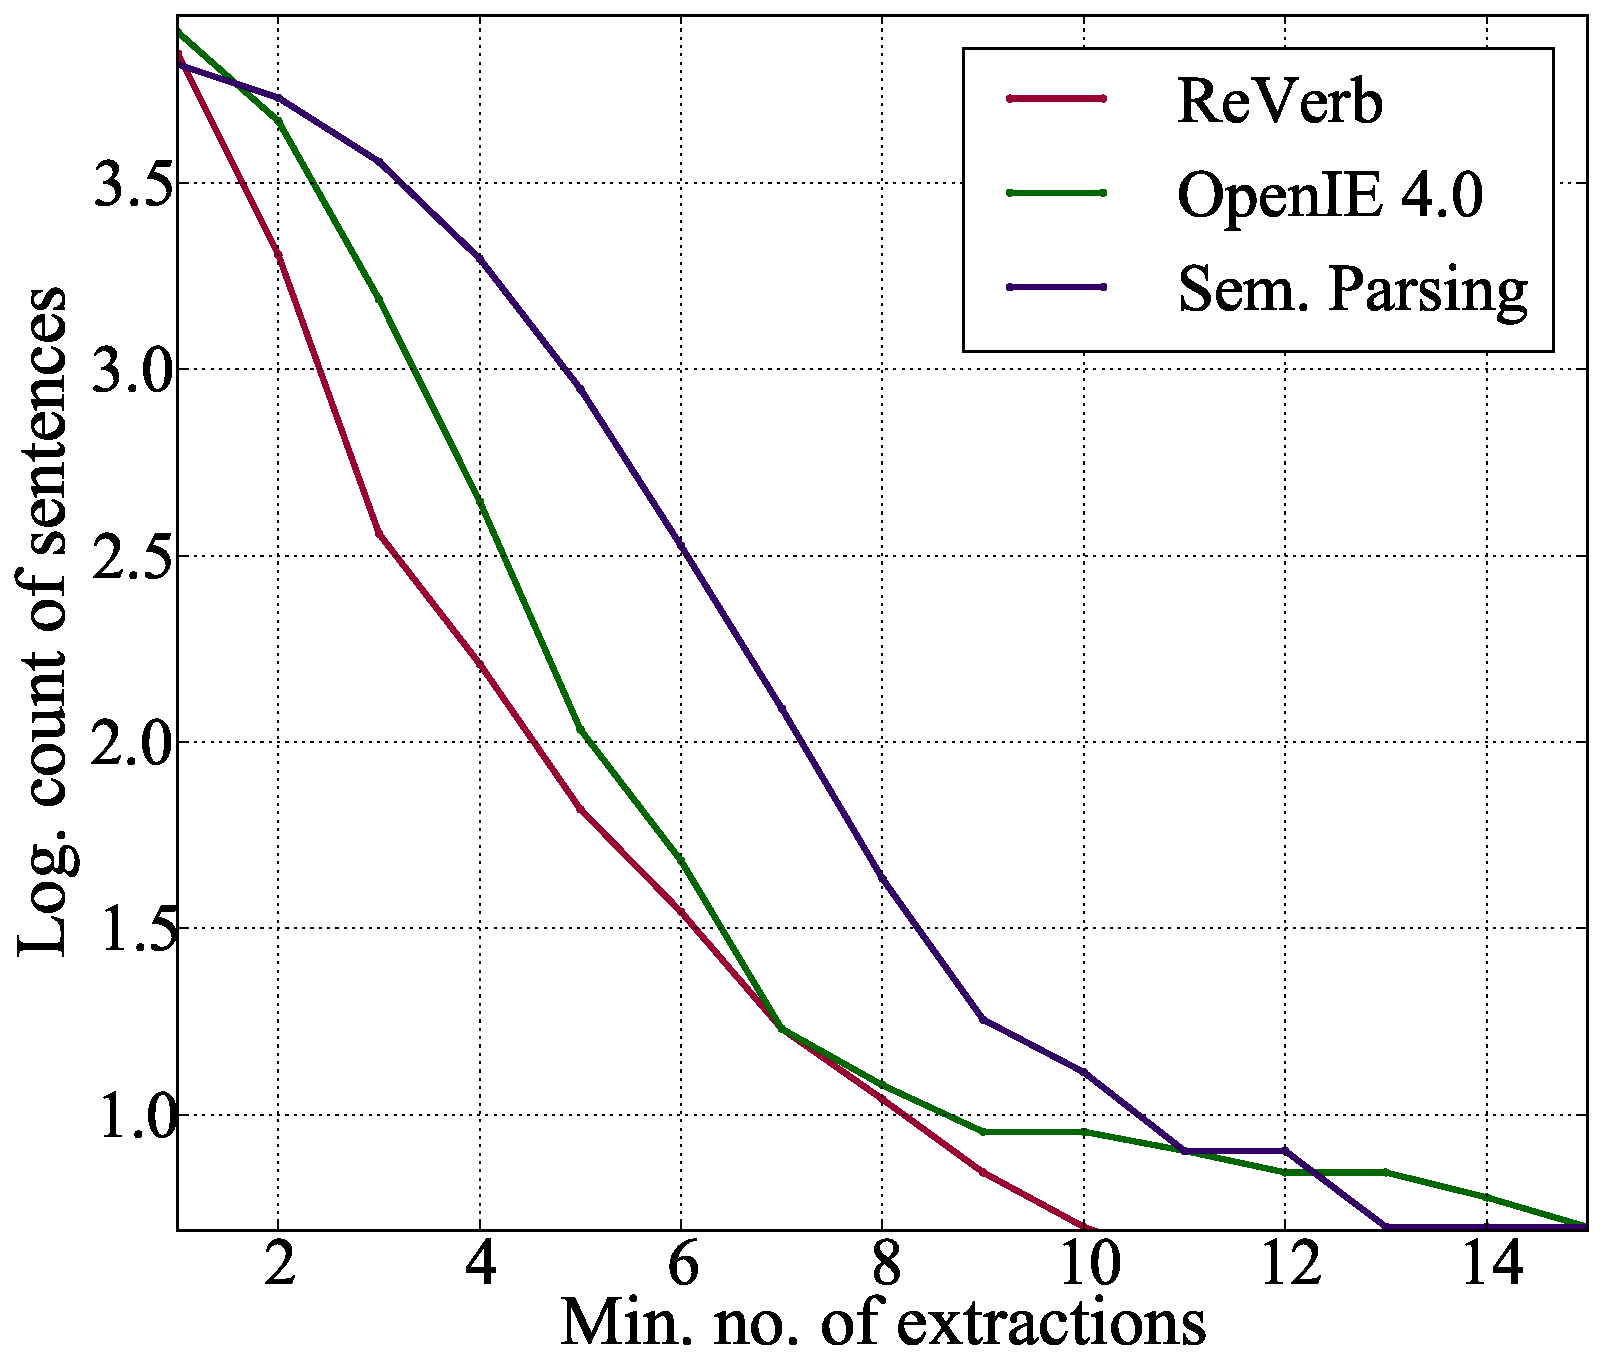
\includegraphics[width=0.45\linewidth]{../../data/results/quantitative/carnatic_music/extrations-per-sentence.pdf}
		 \label{fig:quant-carnatic-sentences}
        }% 
        \qquad
        \subfigure[][Objects]{%
		 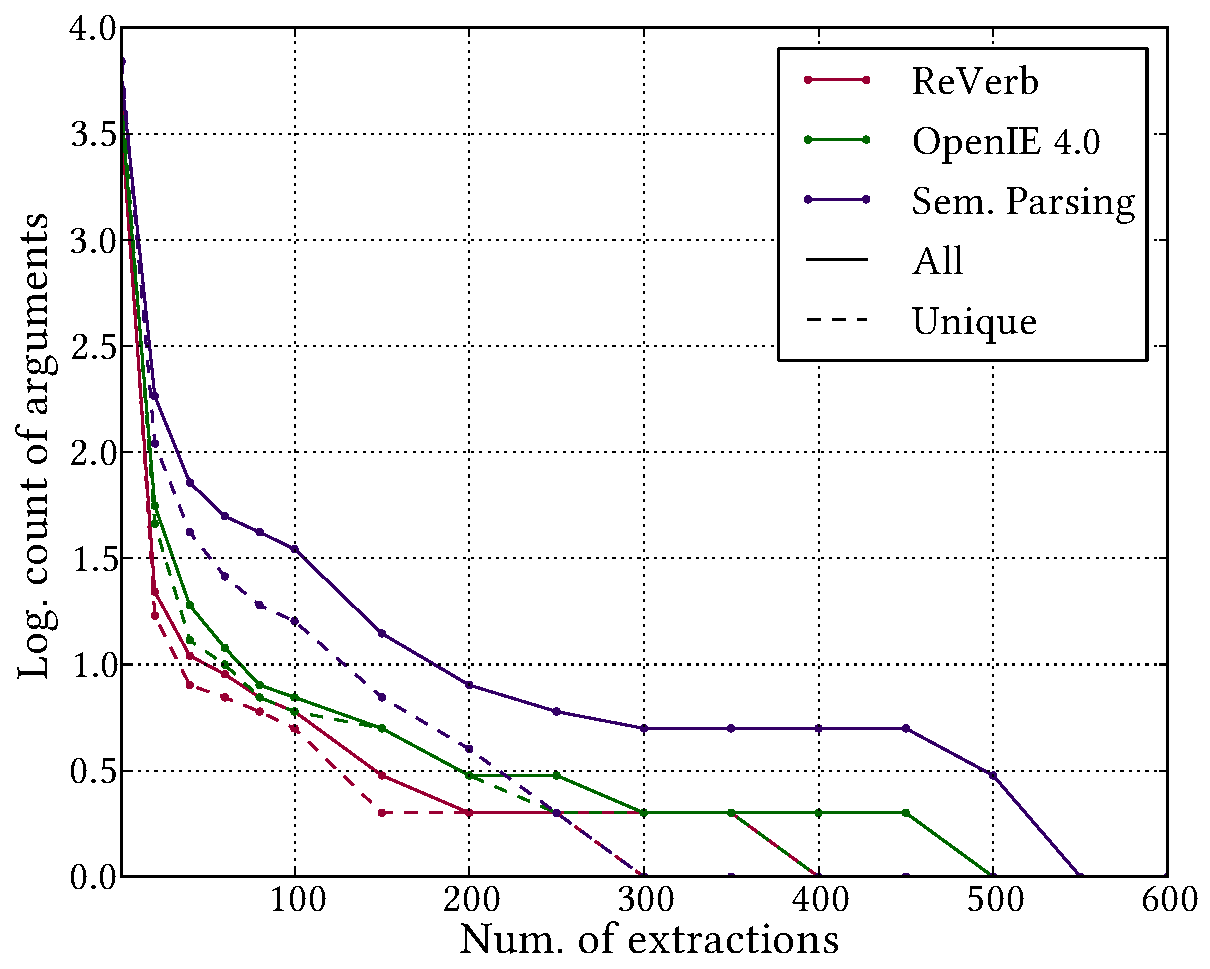
\includegraphics[width=0.45\linewidth]{../../data/results/quantitative/carnatic_music/extrations-per-argument.pdf}
		 \label{fig:quant-carnatic-object}
        }%
        \\
        \subfigure[][Relation types]{%
		 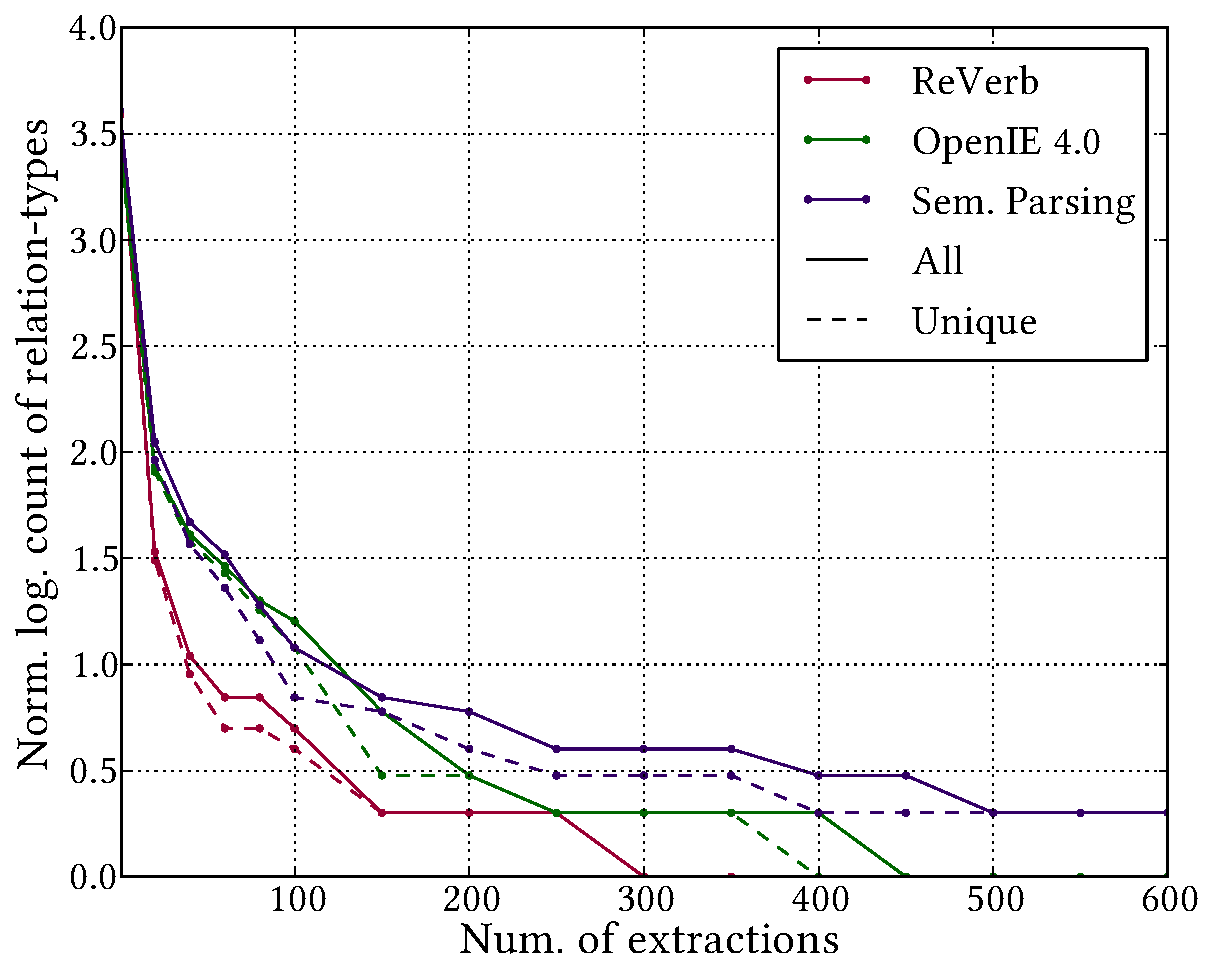
\includegraphics[width=0.45\linewidth]{../../data/results/quantitative/carnatic_music/extrations-per-reltype.pdf}
		 \label{fig:quant-carnatic-reltype}
        }% 
        \qquad
        \subfigure[][Concepts]{%
		 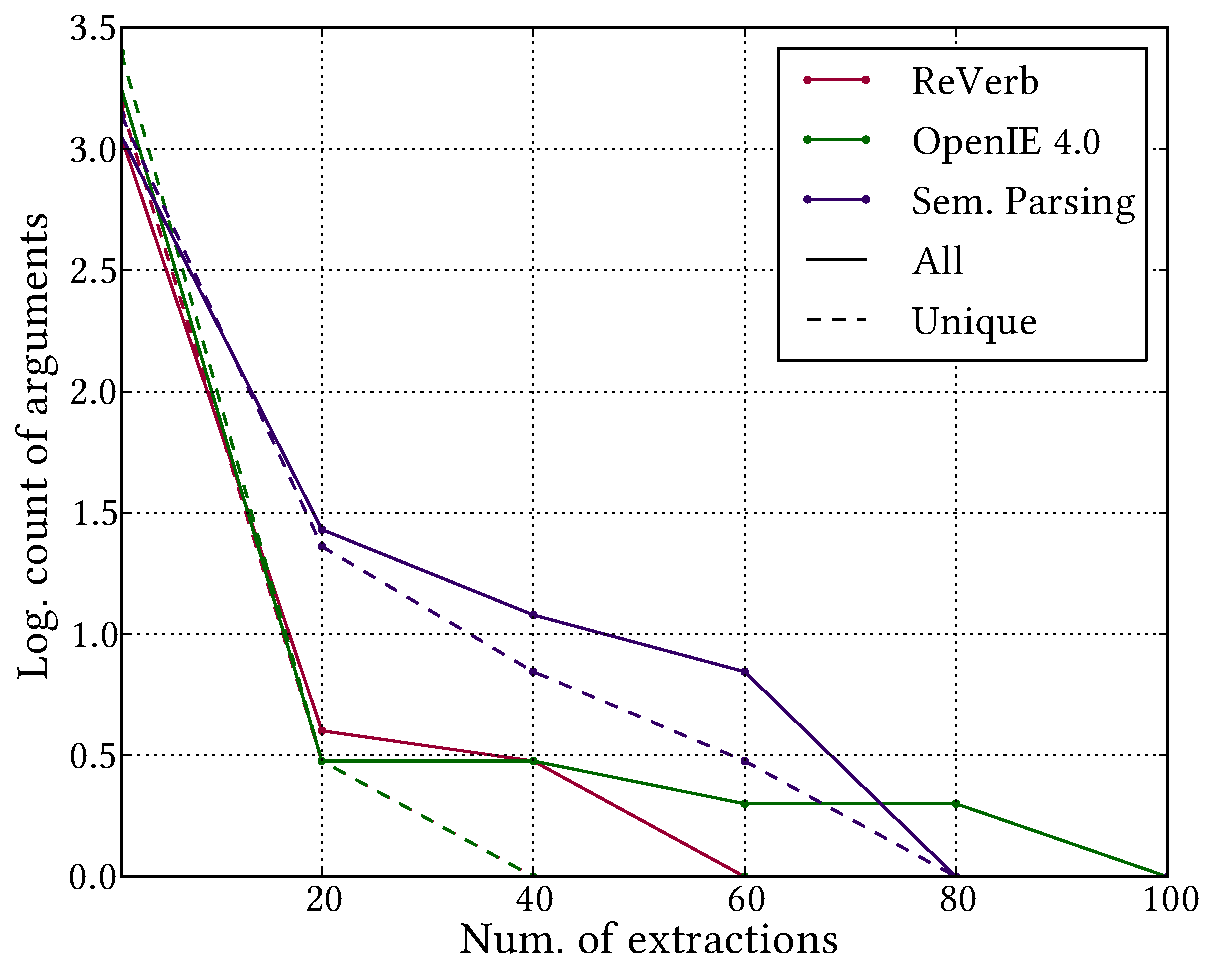
\includegraphics[width=0.45\linewidth]{../../data/results/quantitative/carnatic_music/extrations-per-class.pdf}
		 \label{fig:quant-carnatic-concept}
        }% 
\end{center}
\caption{Distribution of no. of extractions from OIE systems for Carnatic music shown along different \textit{aspects}. For a given number of extractions on x-axis, the y-axis shows the logarithmic count of the instances in the \textit{aspect}, which have at least those many extractions.}
\label{fig:quant-carnatic}
\end{figure}
}

\afterpage{
\begin{figure}[t]
\begin{center} 
        \subfigure[][Sentences]{%
		 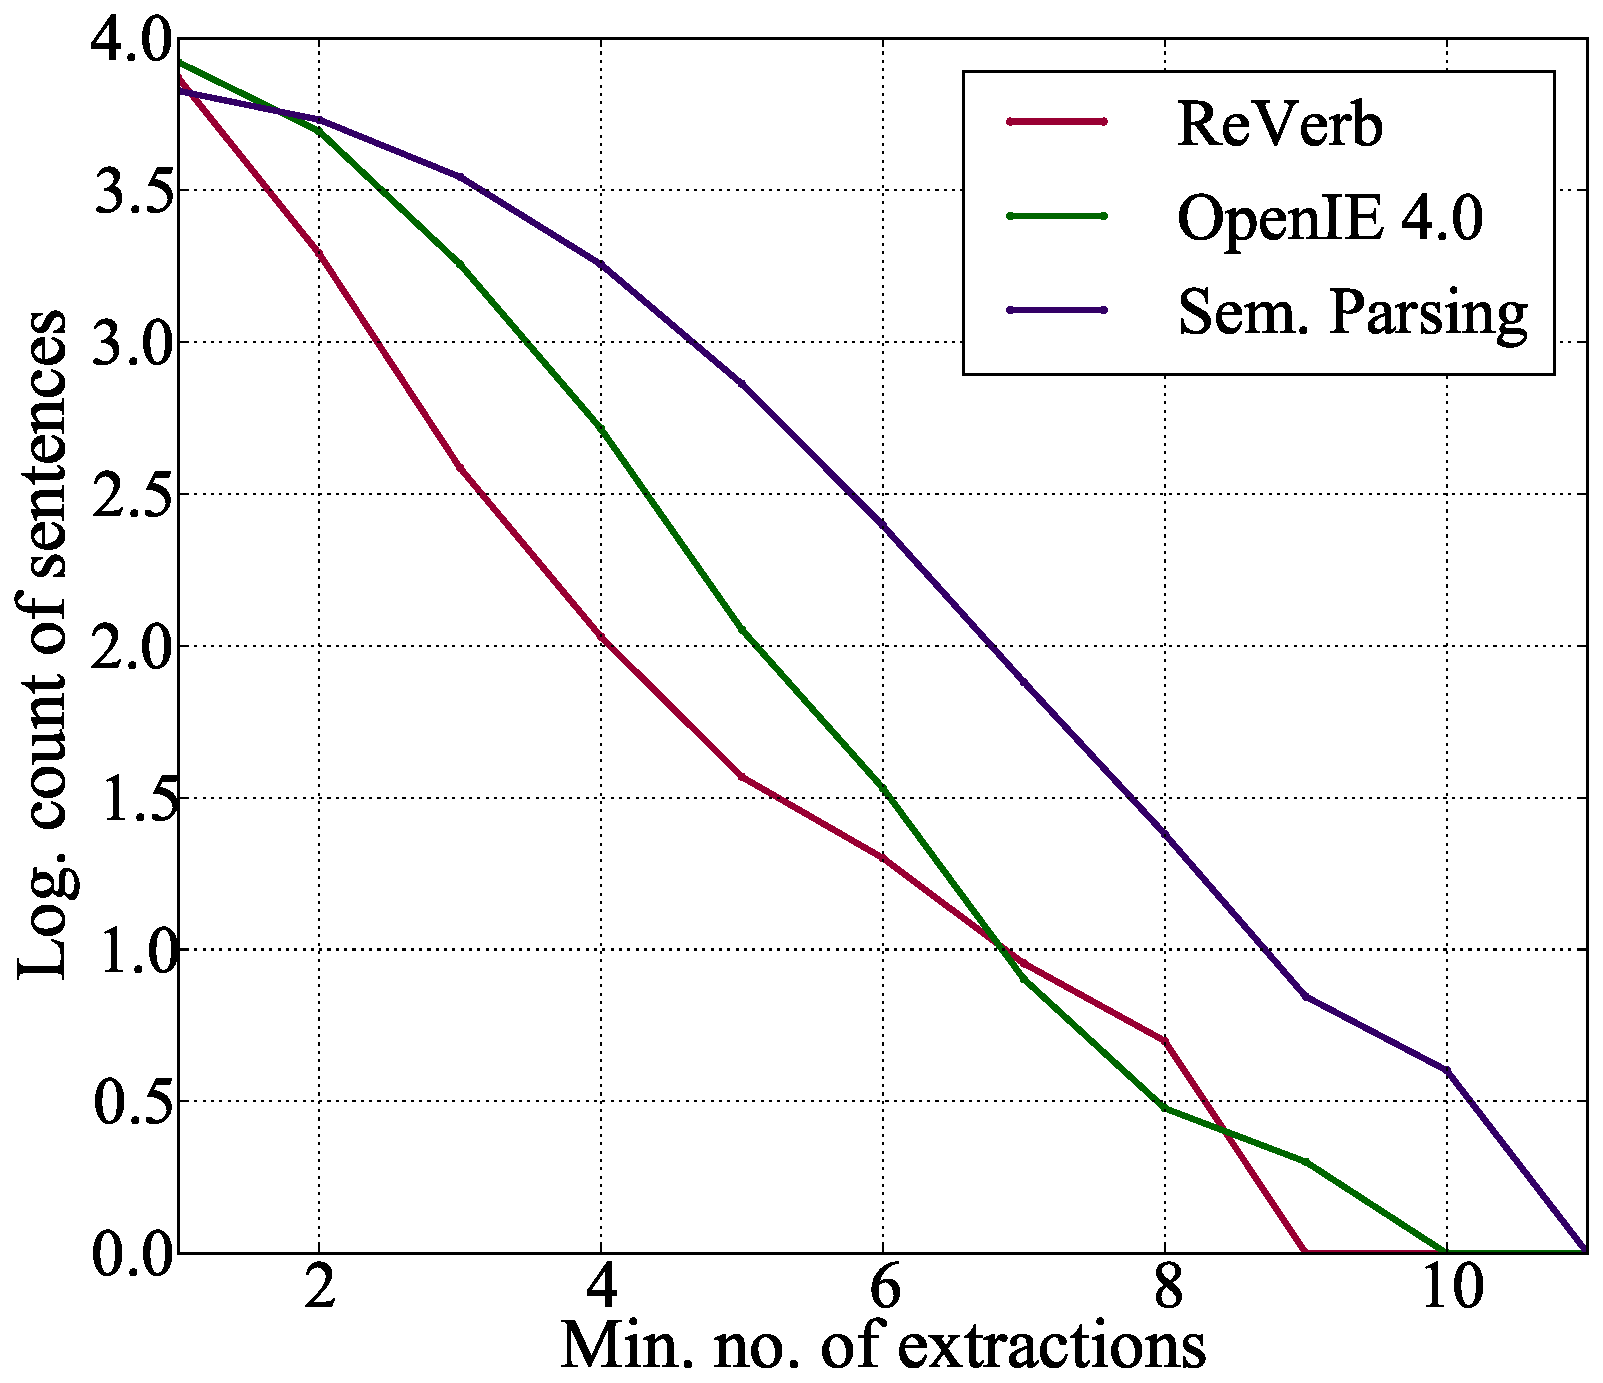
\includegraphics[width=0.45\linewidth]{../../data/results/quantitative/hindustani_music/extrations-per-sentence.pdf}
		 \label{fig:quant-hindustani-sentences}
        }%
        \qquad
        \subfigure[][Objects]{%
		 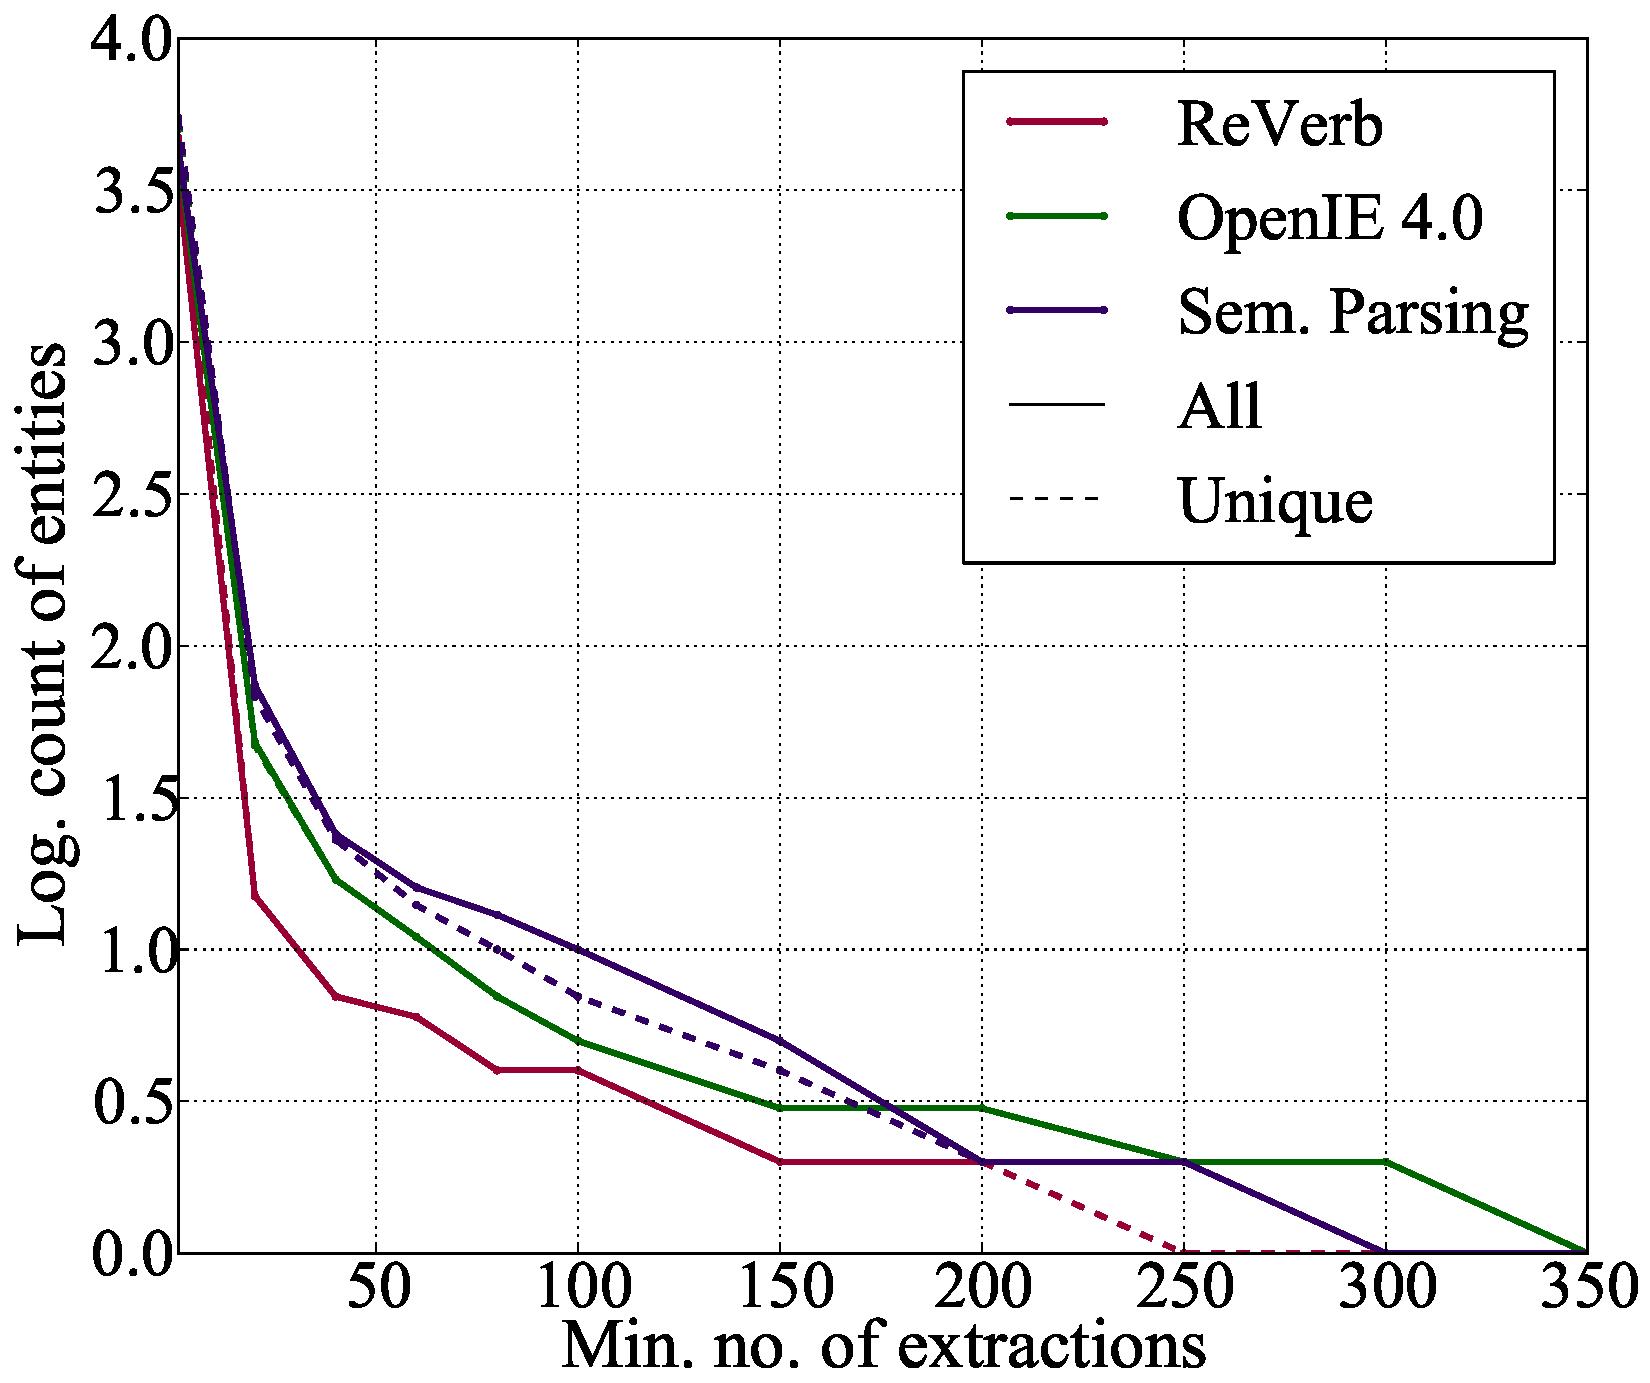
\includegraphics[width=0.45\linewidth]{../../data/results/quantitative/hindustani_music/extrations-per-argument.pdf}
		 \label{fig:quant-hindustani-object}
        }%
        \\
        \subfigure[][Relation types]{%
		 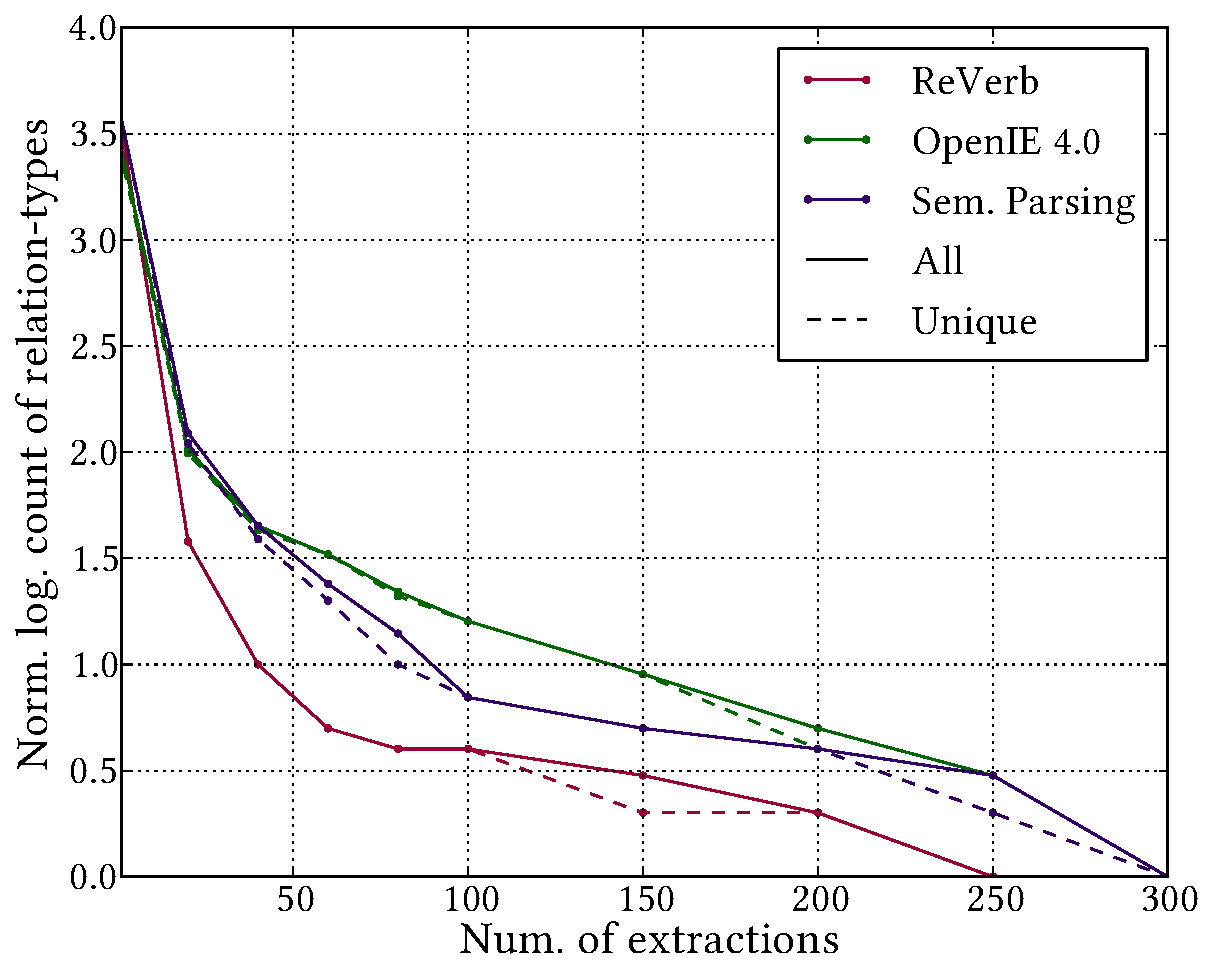
\includegraphics[width=0.45\linewidth]{../../data/results/quantitative/hindustani_music/extrations-per-reltype.pdf}
		 \label{fig:quant-hindustani-reltype}
		}%
        \qquad
        \subfigure[][Concepts]{%
		 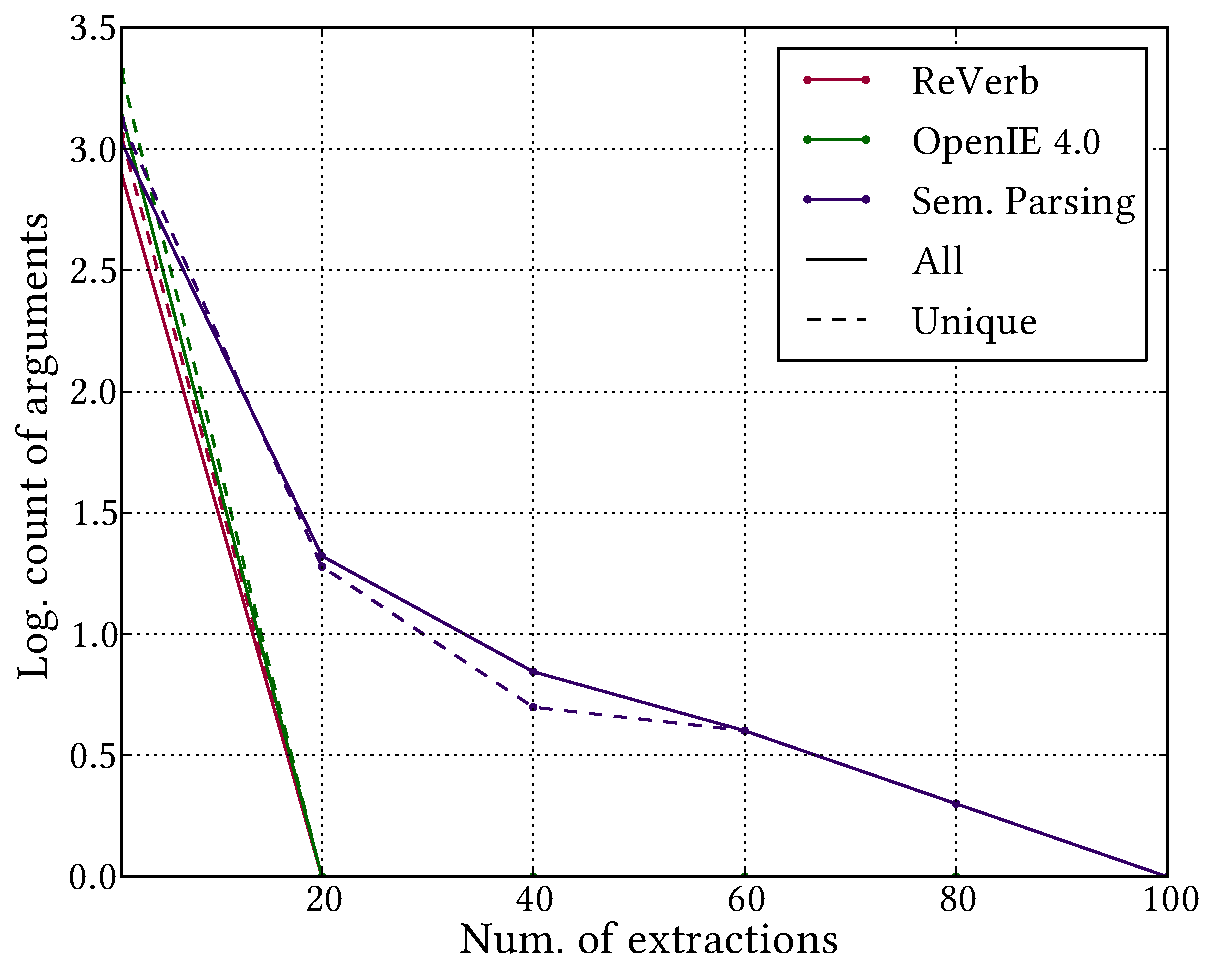
\includegraphics[width=0.45\linewidth]{../../data/results/quantitative/hindustani_music/extrations-per-class.pdf}
		 \label{fig:quant-hindustani-concept}
        }%
\end{center}
\caption{Distribution of no. of extractions from OIE systems for Hindustani music shown along different \textit{aspects}. For a given number of extractions on x-axis, the y-axis shows the logarithmic count of the instances in the \textit{aspect}, which have at least those many extractions.}
\label{fig:quant-hindustani}
\end{figure}
}

\section{Results and discussion}
\label{sec:results}
\subsection{Quantitative assessment}
Figs.~\ref{fig:quant-carnatic-sentences} and \ref{fig:quant-hindustani-sentences} show the distribution of the number of extracted assertions using each of the OIE systems, for sentences in Carnatic and Hindustani music, respectively. Notice that the y-axis is a log scale. Between ReVerb and OpenIE 4.0, the latter seem to perform better, which can be attributed to the noun mediated relations. The semantic parsing based system, however, retrieves substantially more relations per sentence than these two. A tight coupling between syntax and semantics proves to be advantageous in chunking different types of assertions, as well as relating entities far off each other in a given sentence. For instance, in sentences which feature a single subject, but multiple relations (e.g: Chittibabu is a renowned Veena player, born in Kakinada to Ranga Rao and Sundaramma.), it performed thoroughly well compared to others. The difference between their performances for Carnatic and Hindustani music is negligible, which shows that this result is consistent.


Figs.~\ref{fig:quant-carnatic-object} and \ref{fig:quant-hindustani-object} show the corresponding distribution for entities. Recall that we defined an entity to be the subject of a triple. The few entities with a disproportionately high number of extractions are usually the pronouns (despite resolving most of them), followed by musical terms. The semantic parsing based system retrieves slightly more number of assertions per entity compared to OpenIE 4.0, which in turn performs better than ReVerb. We observed some redundancy in assertions for a given entity, which is beneficial as this can be used as a measure of confidence in asserting the corresponding relation. In order to analyze this, we have also plotted the distributions of number of unique extractions for entities (shown in dashed lines in the figures). For Carnatic music, we can observe that the semantic parsing based system retrieves substantially more number of redundant assertions per entity compared to the other two. This difference, however, is less obvious in the case Hindustani music.

Figs.~\ref{fig:quant-carnatic-reltype} and \ref{fig:quant-hindustani-reltype} show the distribution of the number of extracted assertions for the relation types. The results for semantic parsing based system and OpenIE 4.0 are more or less the same, both of which are substantially better than ReVerb. The redundancy in assertions, seen as the difference between the distributions shown by solid and dashed lines, is not as pronounced as it is for entities. The decline in the total number of relation-types as the number of extractions go higher, is less steep than in the case of entities. Unless the vocabulary in the domain is itself limited, this may indicate a slightly better coverage of relation types compared to that of the entities in the domain.


Figs.~\ref{fig:quant-carnatic-concept} and \ref{fig:quant-hindustani-concept} show the distribution of the number of extracted assertions for the concepts. Recall that a concept is defined to be the object of a triple with subsumption relation phrase. The difference between the semantic parsing based system and the other two is quite marked, both for Carnatic and Hindustani music, with the former retrieving more assertions per concept. For Hindustani music, the coverage of concepts in the assertions of ReVerb and OpenIE 4.0 is very low, with no concept having more than 20 assertions.

To summarize, the results indicate that the semantic parsing based system has a better coverage of entities, concepts and relation types of the domain than OpenIE 4.0, which is followed by ReVerb. It also retrieves more assertions per sentence compared to the other two. Note that this section has only provided the quantitative information, which by no means is complete in itself. The results we discuss in the following section complement these providing qualitative observations along the same dimensions (i.e., entities, concepts and relation types).

\subsection{Qualitative assessment}
In this section, we present the results for various tasks in the ontologization of Indian art music domain: concept identification, entity identification and semantic relation extraction.

\paragraph{Concept identification.}
Recall that we define candidate concepts to be the collection of objects from the triples with subsumption relation type. We map these to the concepts in the ontologies as described in sec.~\ref{sec:framework}. Table.~\ref{tab:concept_identification} shows the number of concepts in the ontolgies for each music, and the number of concepts mapped from the assertions of the OIE systems. These results are consistent with our earlier observations of the results shown in figs.~\ref{fig:quant-carnatic-concept} and~\ref{fig:quant-hindustani-concept}.
\begin{table}
 \begin{center}
 \begin{tabularx}{0.9\textwidth}{X X X X X}
 \noalign{\hrule height 1.1pt}
  \textbf{Music} & \textbf{\#Ontology} & \textbf{\#ReVerb} & \textbf{\#OpenIE 4.0} & \textbf{\#Sem. Parsing}\\
  \hline
  Carnatic  & 53 & 4 & 4 & 22 \\
  Hindustani  & 55 & 1 & 2 & 9 \\
 \noalign{\hrule height 1.1pt}
 \end{tabularx}
\end{center}
\caption{The number of concepts in the ontologies for each music, and those mapped from the assertions of the OIE systems.}
\label{tab:concept_identification}
\end{table}

%\afterpage{
\begin{figure}[t!]
\begin{center}
        \subfigure[][Overlap with reference data.]{%
		 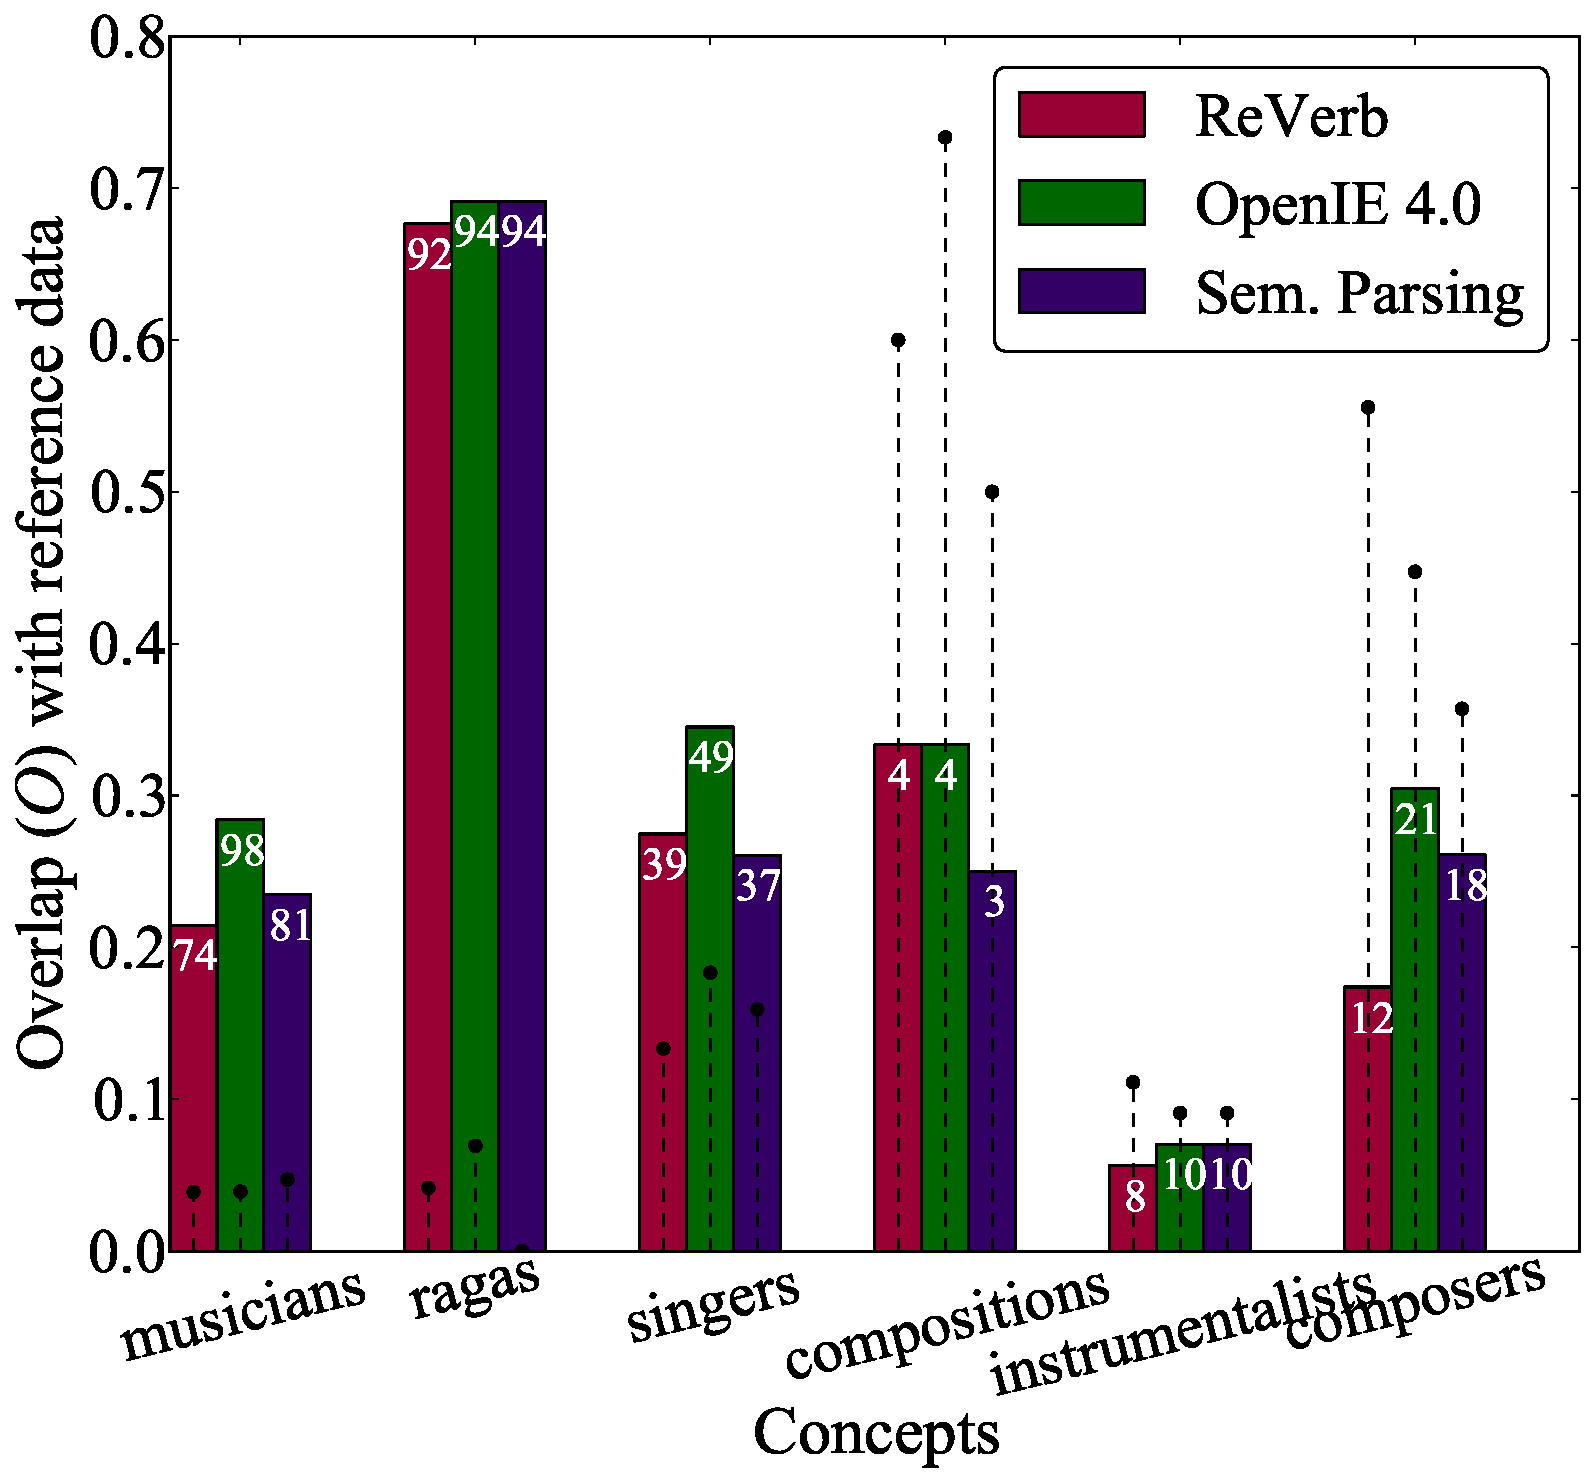
\includegraphics[width=0.45\linewidth]{../../data/results/qualitative/entity-identification/rule-based/carnatic_music/class-agreement-with-wikipedia.pdf}
		 \label{fig:qual-object-rulebased-carnatic-wikipedia}
        }% 
        \qquad
        \subfigure[][Inter-system agreement for residual entity cadidates.]{%
		 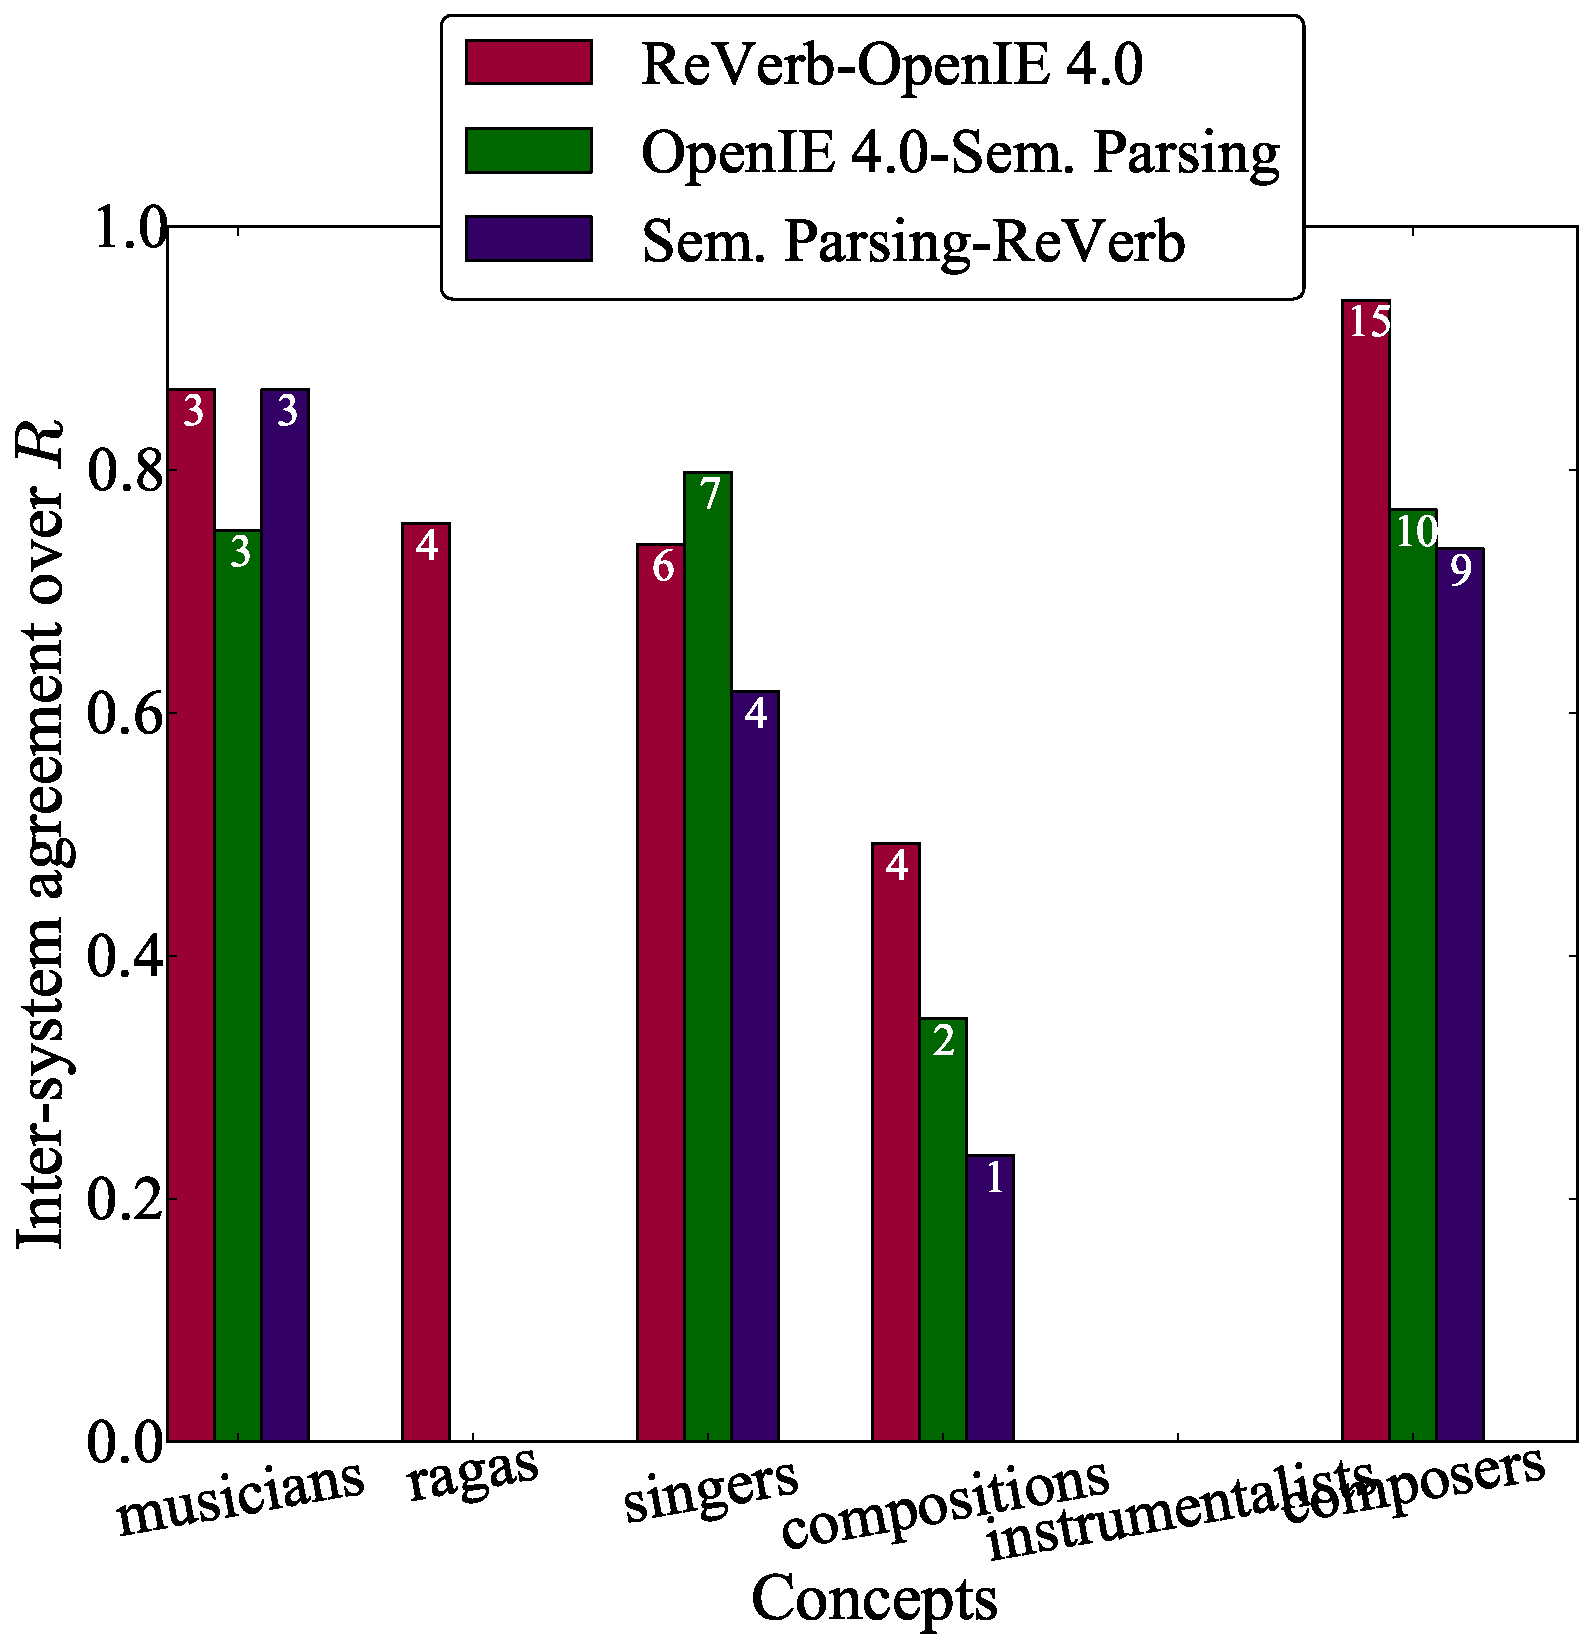
\includegraphics[width=0.45\linewidth]{../../data/results/qualitative/entity-identification/rule-based/carnatic_music/class-agreement-inter-method.pdf}
		 \label{fig:qual-object-rulebased-carnatic-inter}
		}%
		\\
        \subfigure[][Overlap with reference data.]{%
		 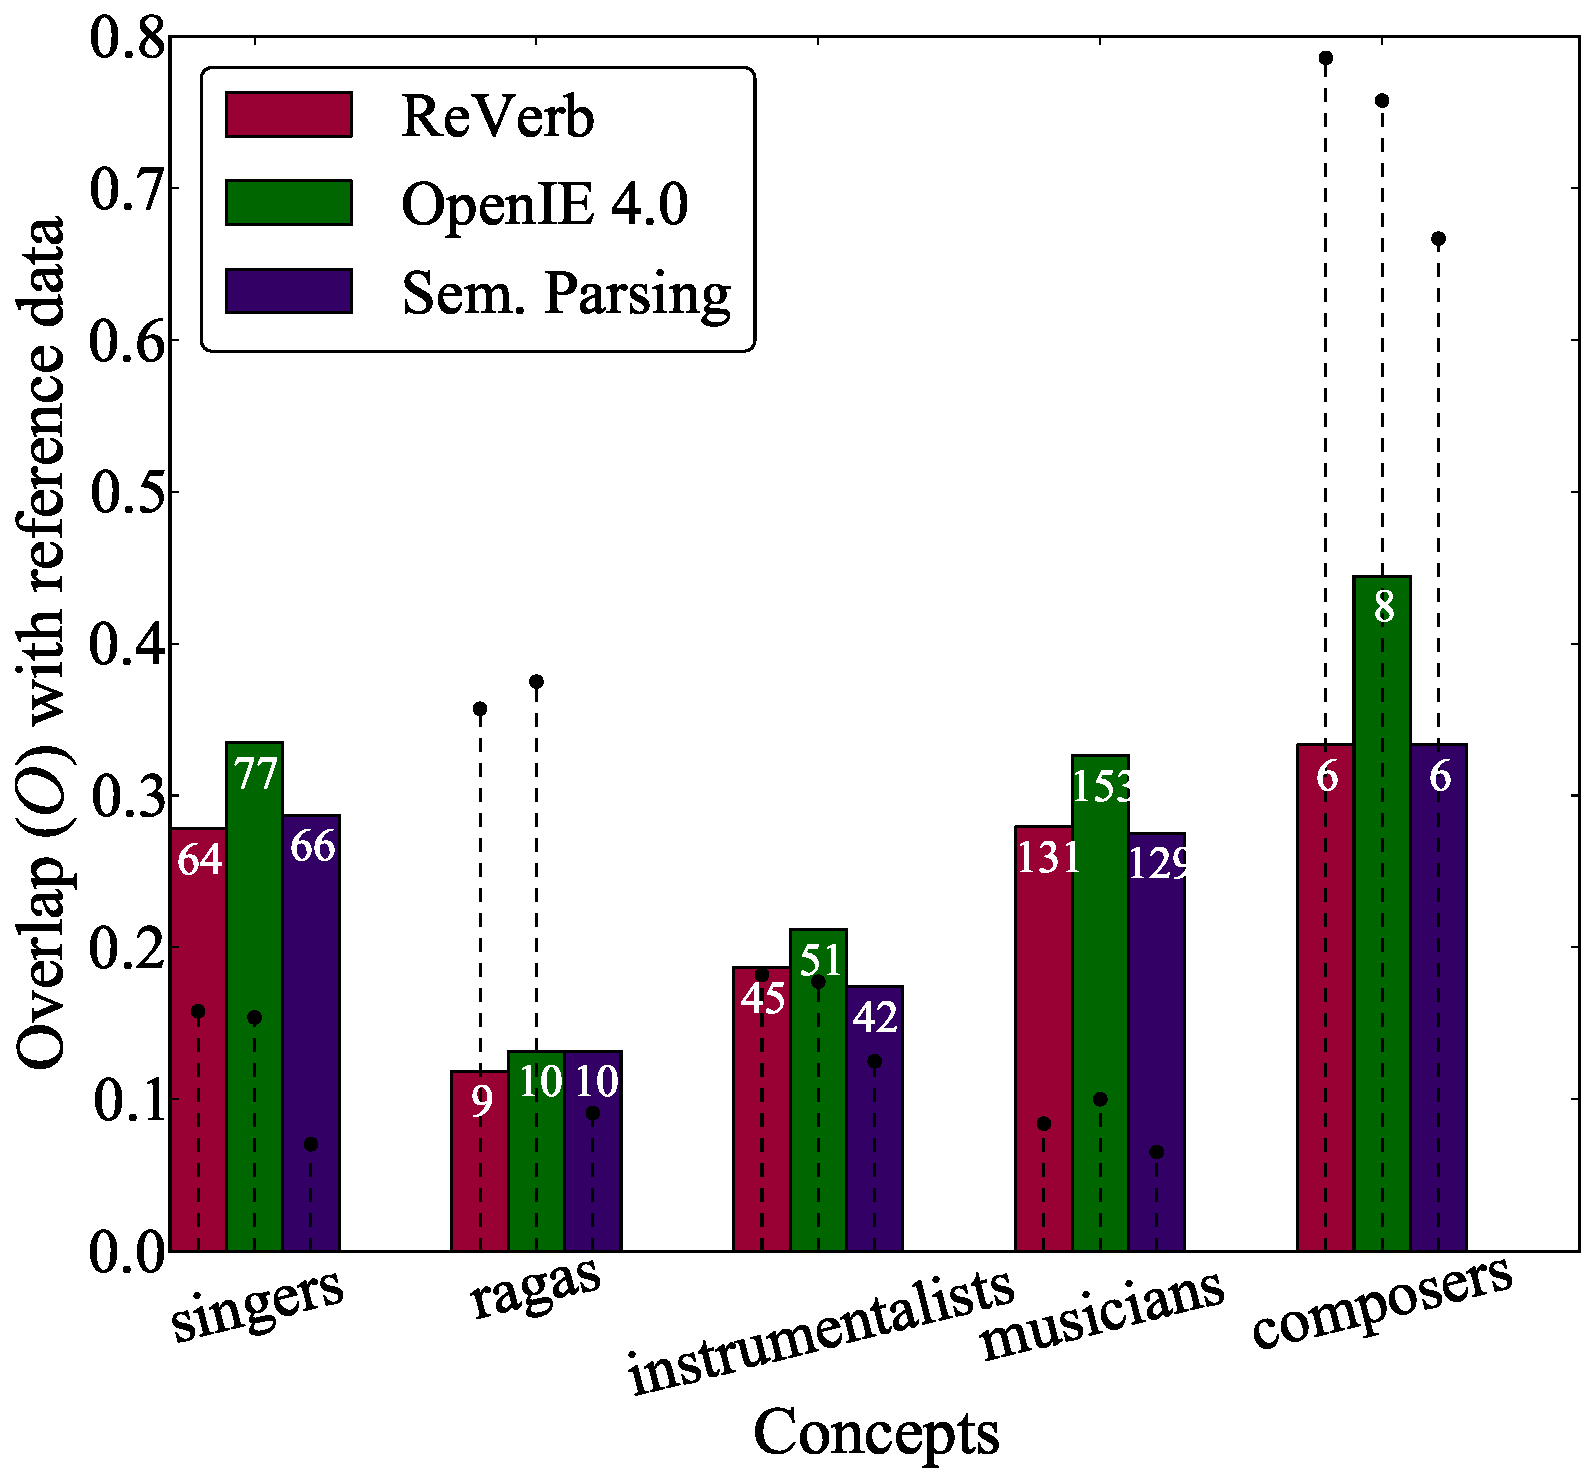
\includegraphics[width=0.45\linewidth]{../../data/results/qualitative/entity-identification/rule-based/hindustani_music/class-agreement-with-wikipedia.pdf}
		 \label{fig:qual-object-rulebased-hindustani-wikipedia}
        }%
        \qquad
        \subfigure[][Inter-system agreement for residual entity cadidates.]{%
		 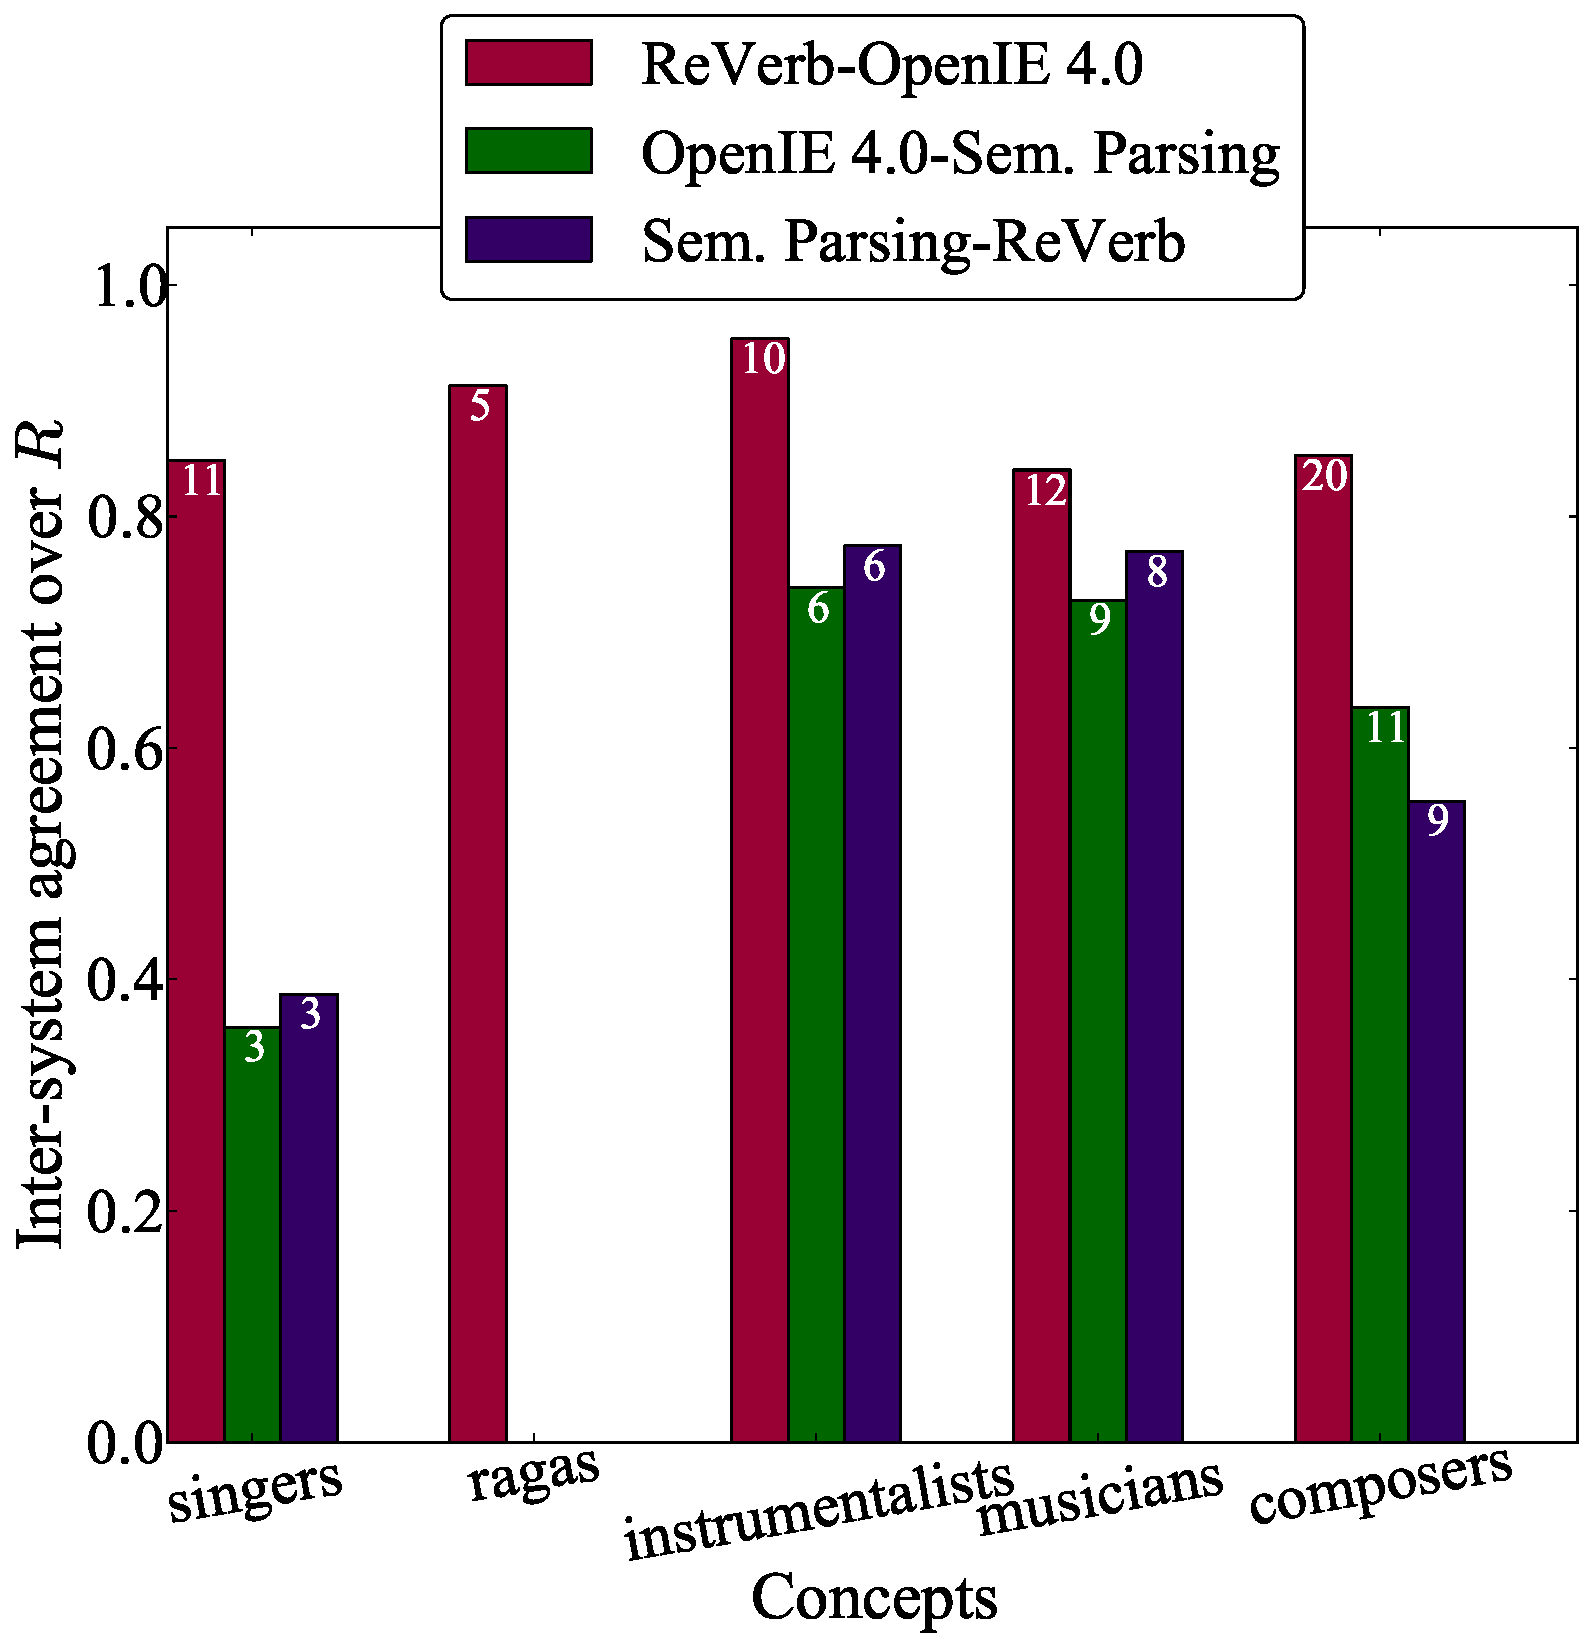
\includegraphics[width=0.45\linewidth]{../../data/results/qualitative/entity-identification/rule-based/hindustani_music/class-agreement-inter-method.pdf}
		 \label{fig:qual-object-rulebased-hindustani-inter}
        }%
\end{center}
\caption{Results for rule-based concept assignment of entities identified in Carnatic (top) and Hindustani (bottom) music.}
\label{fig:qual-object-rulebased}
\end{figure}
%}

\paragraph{Entity identification.}
The first subtask in this part is to find the entities in the domain. The candidate entities from each OIE system are defined to be the collection of subjects from all its triples. Table.~\ref{tab:object_identification} shows the total number of entities in the reference data taken from Wikipedia for each music, and the number of entities in the intersection of these with the candidate entities of each OIE system. There is no marked difference between the results, with nearly all the systems having about 60\% of the entities from reference data in their assertions. However, it is observed that these correspond to only about 7\% of all the possible candidate entities.
\begin{table}
 \begin{center}
 \begin{tabularx}{0.9\textwidth}{X X X X X}
 \noalign{\hrule height 1.1pt}
  \textbf{Music} & \textbf{\#Reference} & \textbf{\#ReVerb} & \textbf{\#OpenIE 4.0} & \textbf{\#Sem. Parsing}\\
  \hline
  Carnatic  & 618 & 349 & 364 & 364 \\
  Hindustani  & 697 & 396 & 410 & 399 \\
 \noalign{\hrule height 1.1pt}
 \end{tabularx}
\end{center}
\caption{The number of entities in the reference data for each music, and those identified using the OIE systems.}
\label{tab:object_identification}
\end{table}

For the second subtask of entity identification, i.e., assigning entities to concepts, we have considered those concepts from our ontology for which there is a corresponding category on Wikipedia, each having at least 20 pages. This was done to avoid manual labeling of entities. We found 5 such concepts for Hindustani music: musicians, singers, instrumentalists, composers and ragas\footnote{Raga is the melodic framework for both the Indian art music traditions.}. For Carnatic music, in addition to these, we have found another concept: compositions. As discussed, we evaluate this task using two methods: rule-based and bootstrapping-based method.

Figs.~\ref{fig:qual-object-rulebased-carnatic-wikipedia} and \ref{fig:qual-object-rulebased-hindustani-wikipedia} show the overlap ($O$, see eq.~\ref{eq:overlap}) on rule-based concept assignment for entities found in Carnatic and Hindustani music using the OIE systems. The stem plots in the figures show residual portion of entities ($R$). The most notable performances are seen for the raga concept in Carnatic music. This can be attributed to two specific reasons: most Carnatic ragas on Wikipedia are described using a template, and the terminology consists mainly of Sanskrit terms which set them apart from the rest (mainly people). On the other hand, the description for Hindustani ragas varied a lot from raga to raga, and often the Sanskrit terms are inconsistently romanized making it hard for OIE systems to retrieve meaningful assertions. In theory, there is a template for almost every category, but there is a lot of variability, such as this, in describing the corresponding entities, except in the case of Carnatic ragas. OpenIE 4.0 seems to perform slightly better in terms of overlap, compared to the semantic parsing based system and ReVerb.

\afterpage{
\begin{figure}[p]
\begin{center}
        \subfigure[][Musicians]{%
		 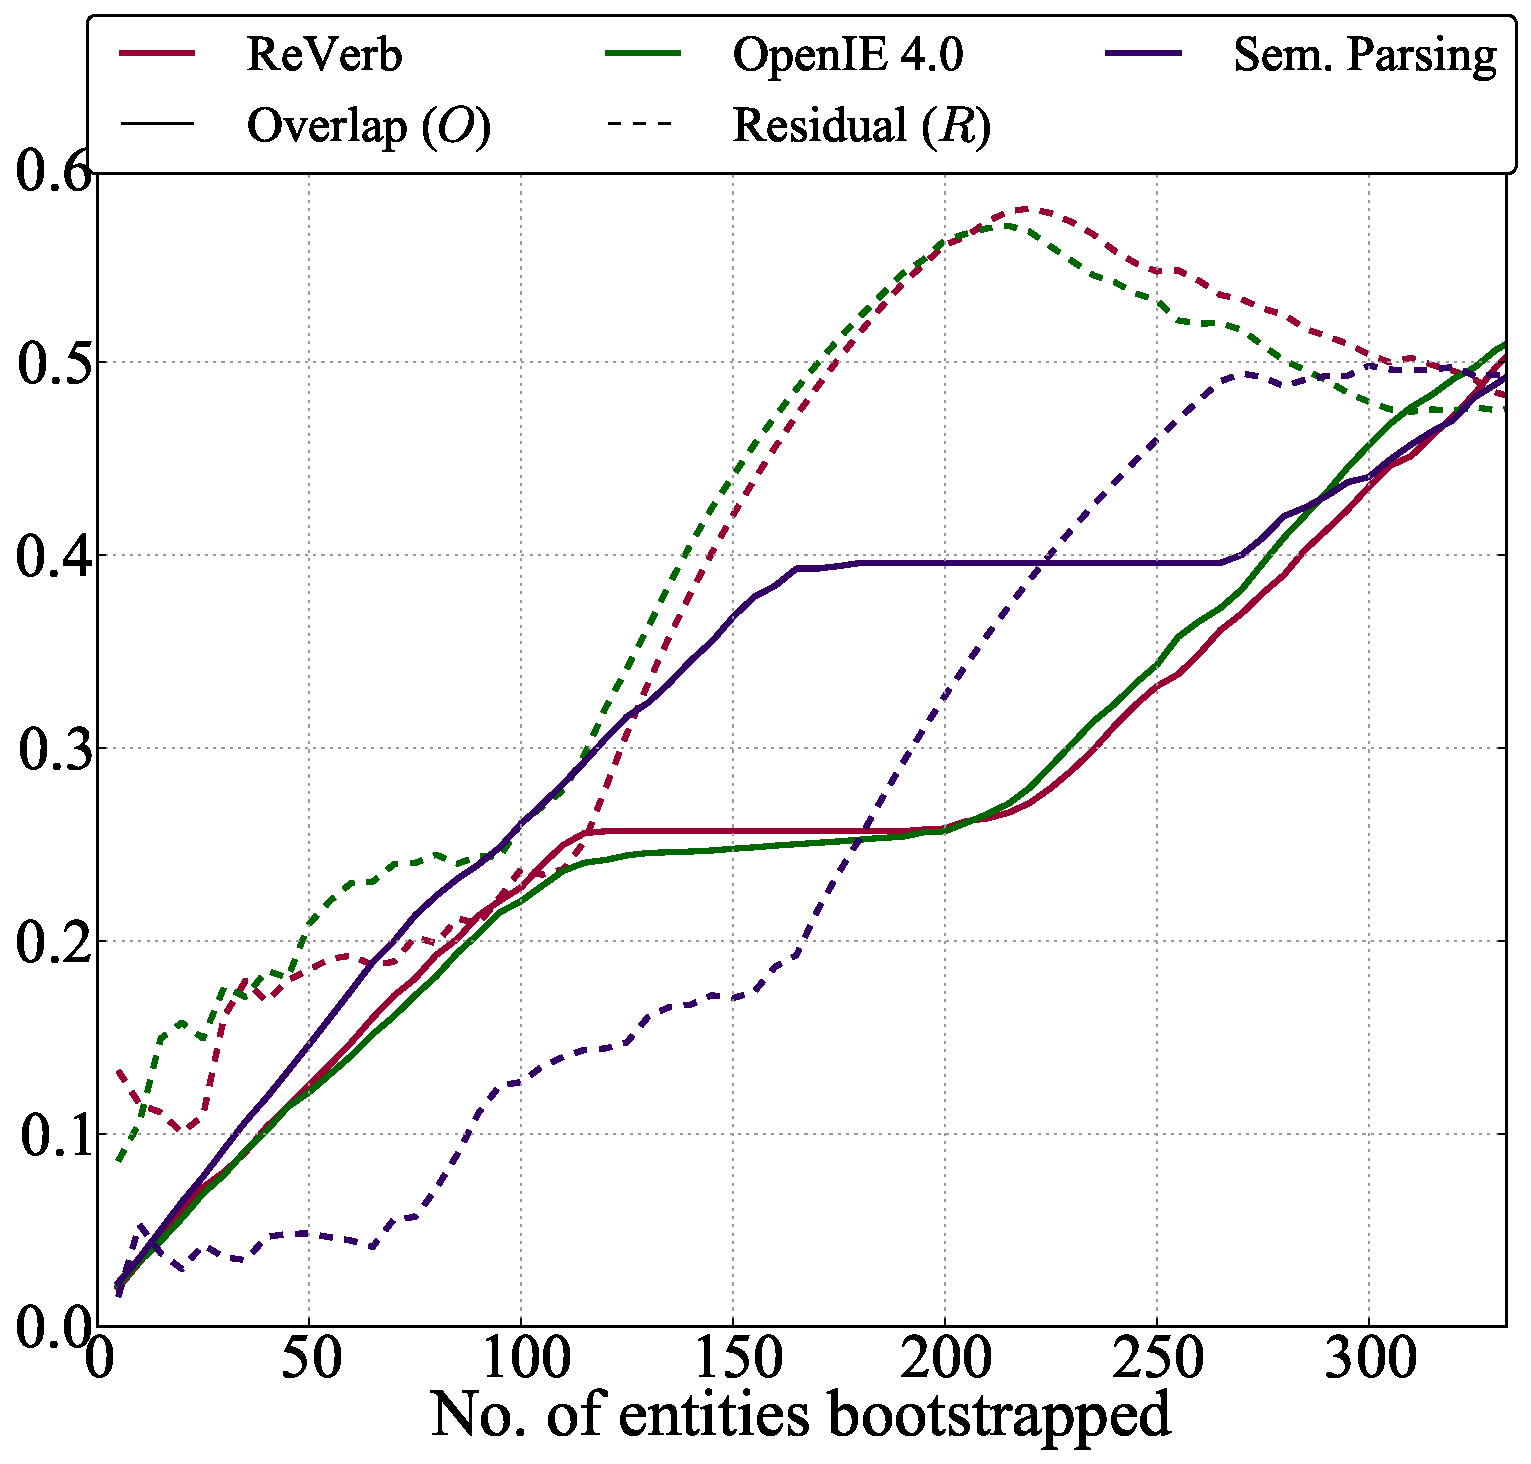
\includegraphics[width=0.45\linewidth]{../../data/results/qualitative/entity-identification/bootstrapping/carnatic_music/carnatic_musicians.pdf}
		 \label{fig:qual-object-bootstrapping-carnatic-musicians}
        }% 
        \qquad
        \subfigure[][Composers]{%
		 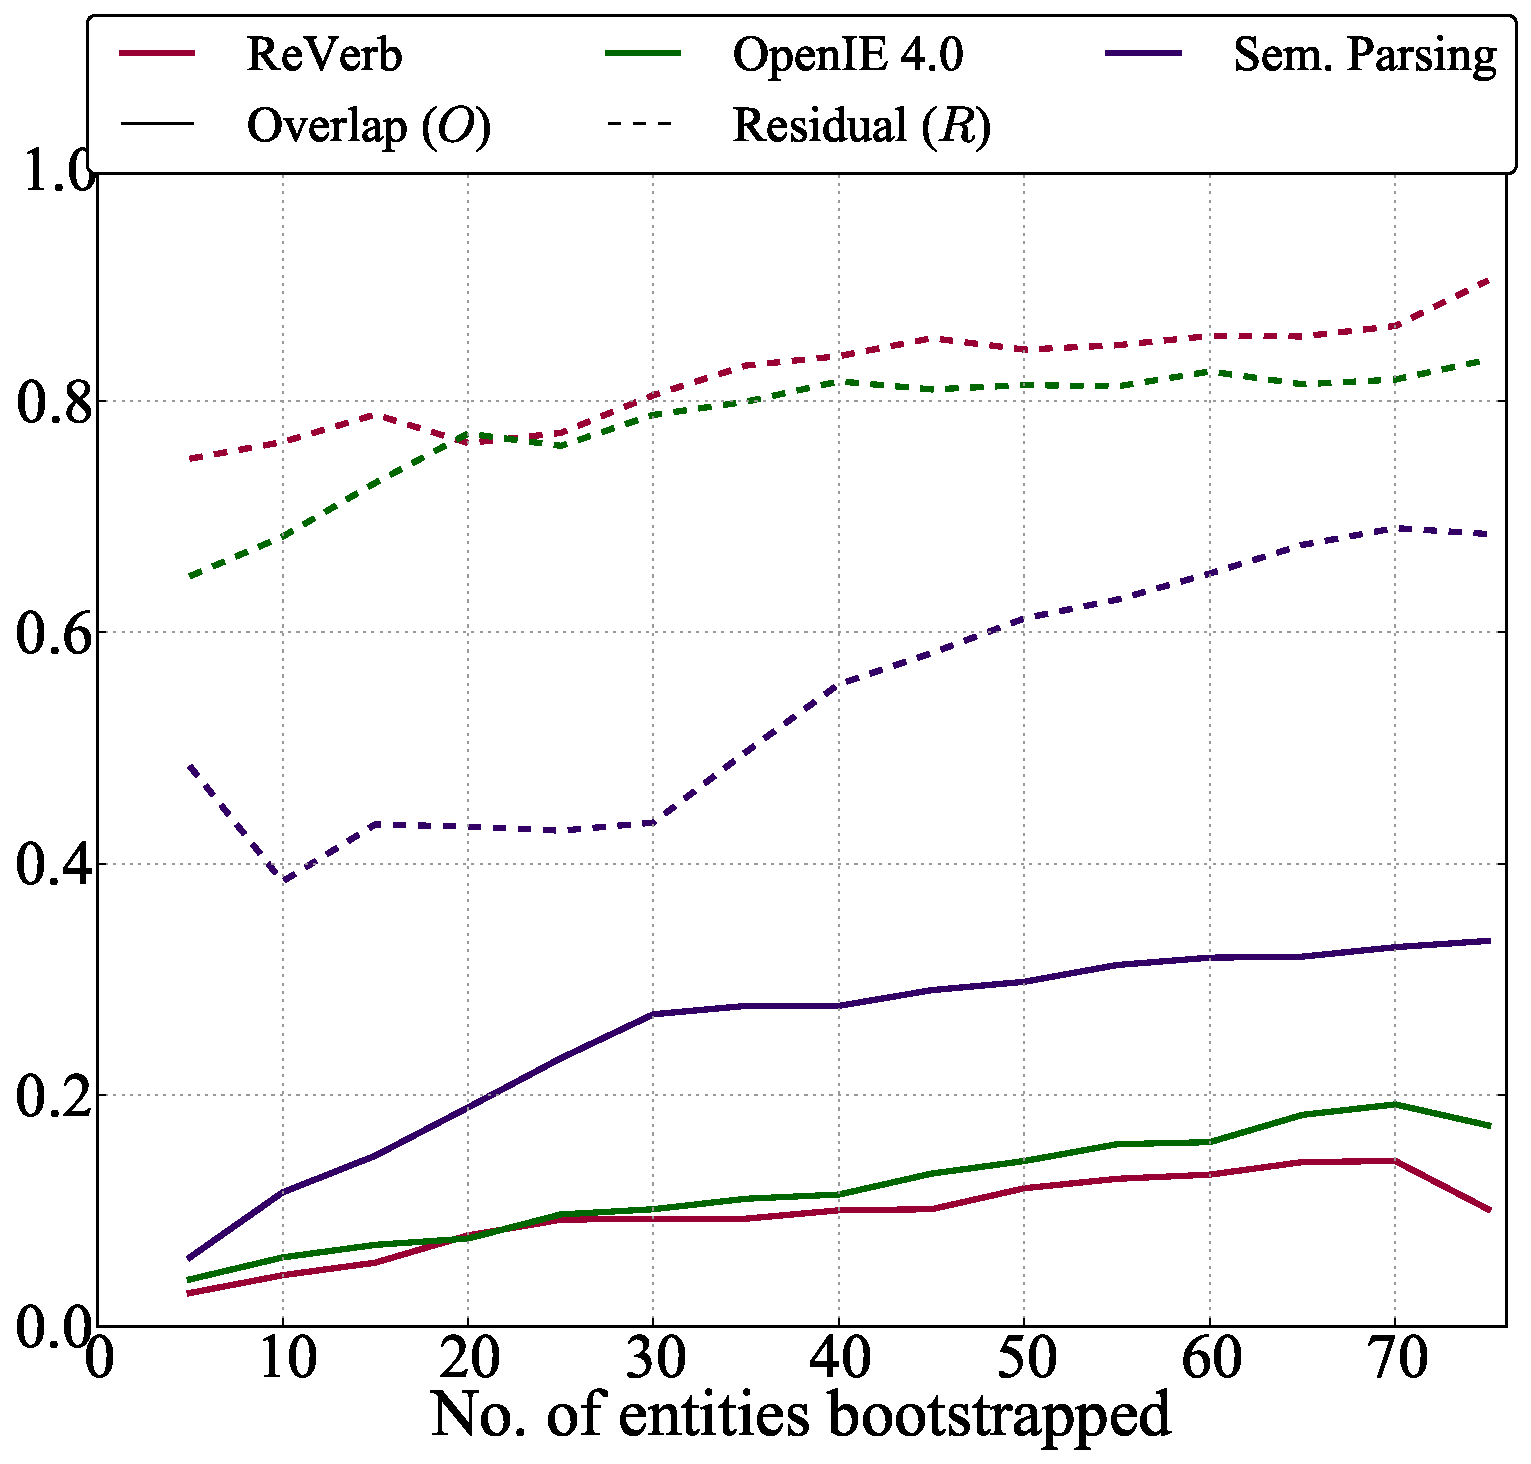
\includegraphics[width=0.45\linewidth]{../../data/results/qualitative/entity-identification/bootstrapping/carnatic_music/carnatic_composers.pdf}
		 \label{fig:qual-object-bootstrapping-carnatic-composers}
        }%
        \\
        \subfigure[][Instrumentalists]{%
		 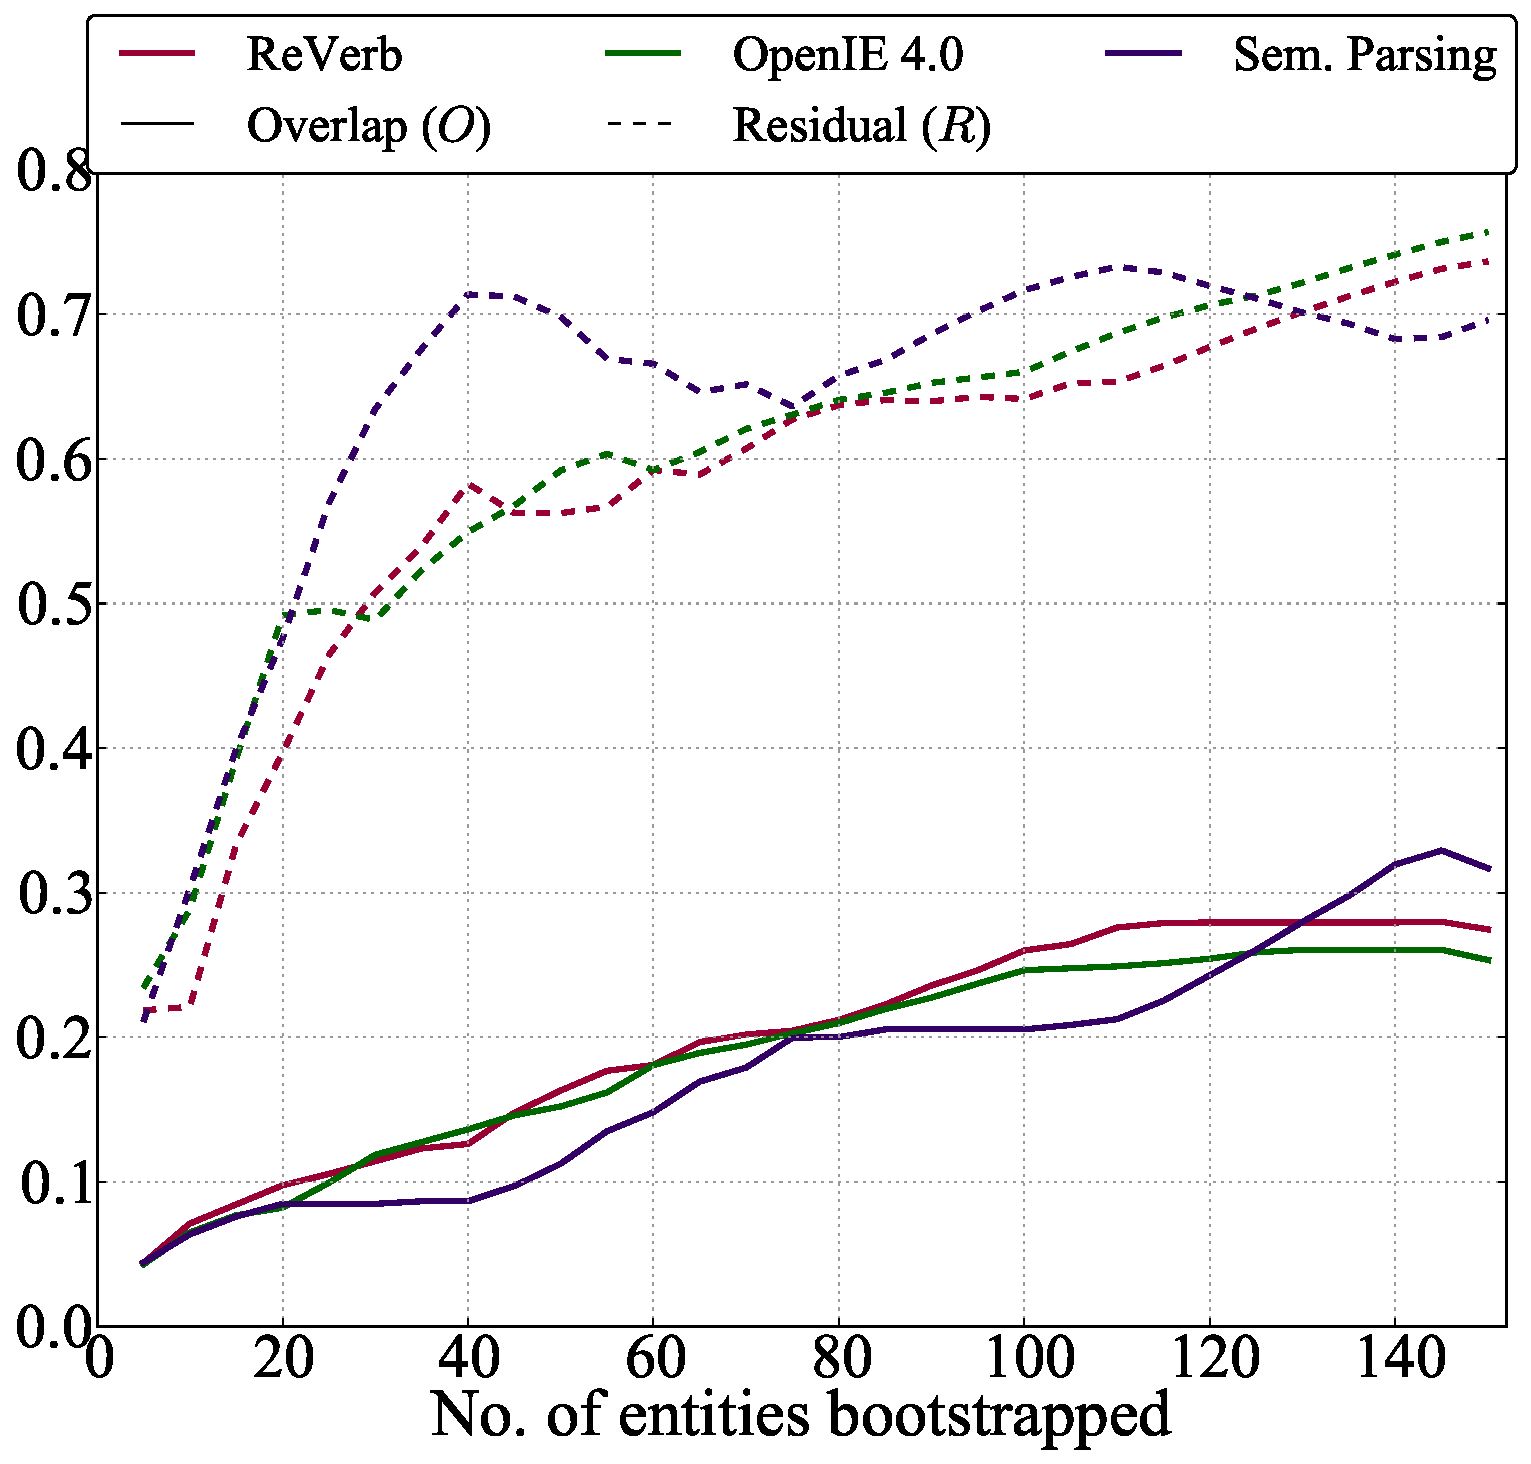
\includegraphics[width=0.45\linewidth]{../../data/results/qualitative/entity-identification/bootstrapping/carnatic_music/carnatic_instrumentalists.pdf}
		 \label{fig:qual-object-bootstrapping-carnatic-instrumentalists}
        }% 
        \qquad
        \subfigure[][Singers]{%
		 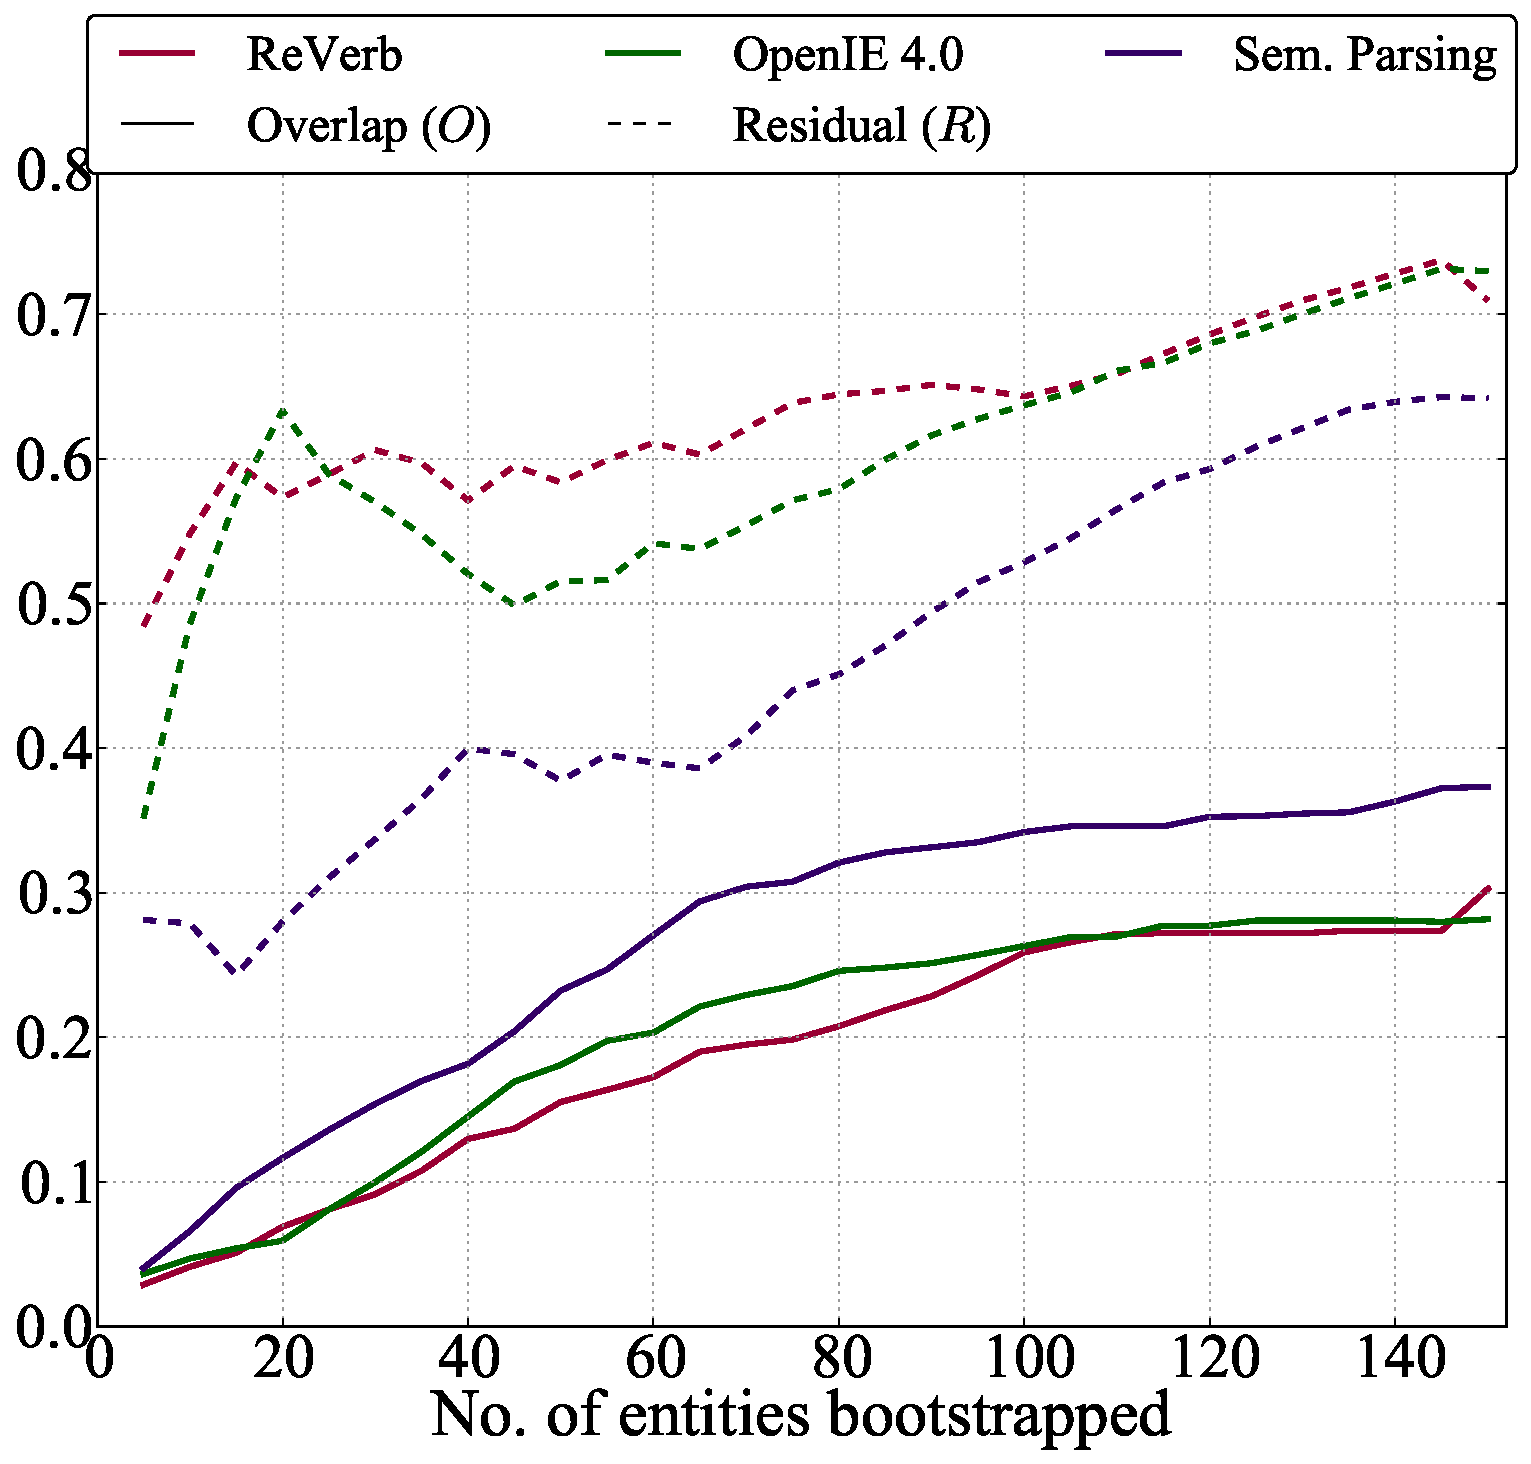
\includegraphics[width=0.45\linewidth]{../../data/results/qualitative/entity-identification/bootstrapping/carnatic_music/carnatic_singers.pdf}
		 \label{fig:qual-object-bootstrapping-carnatic-singers}
        }%
        \\
        \subfigure[][Ragas]{%
		 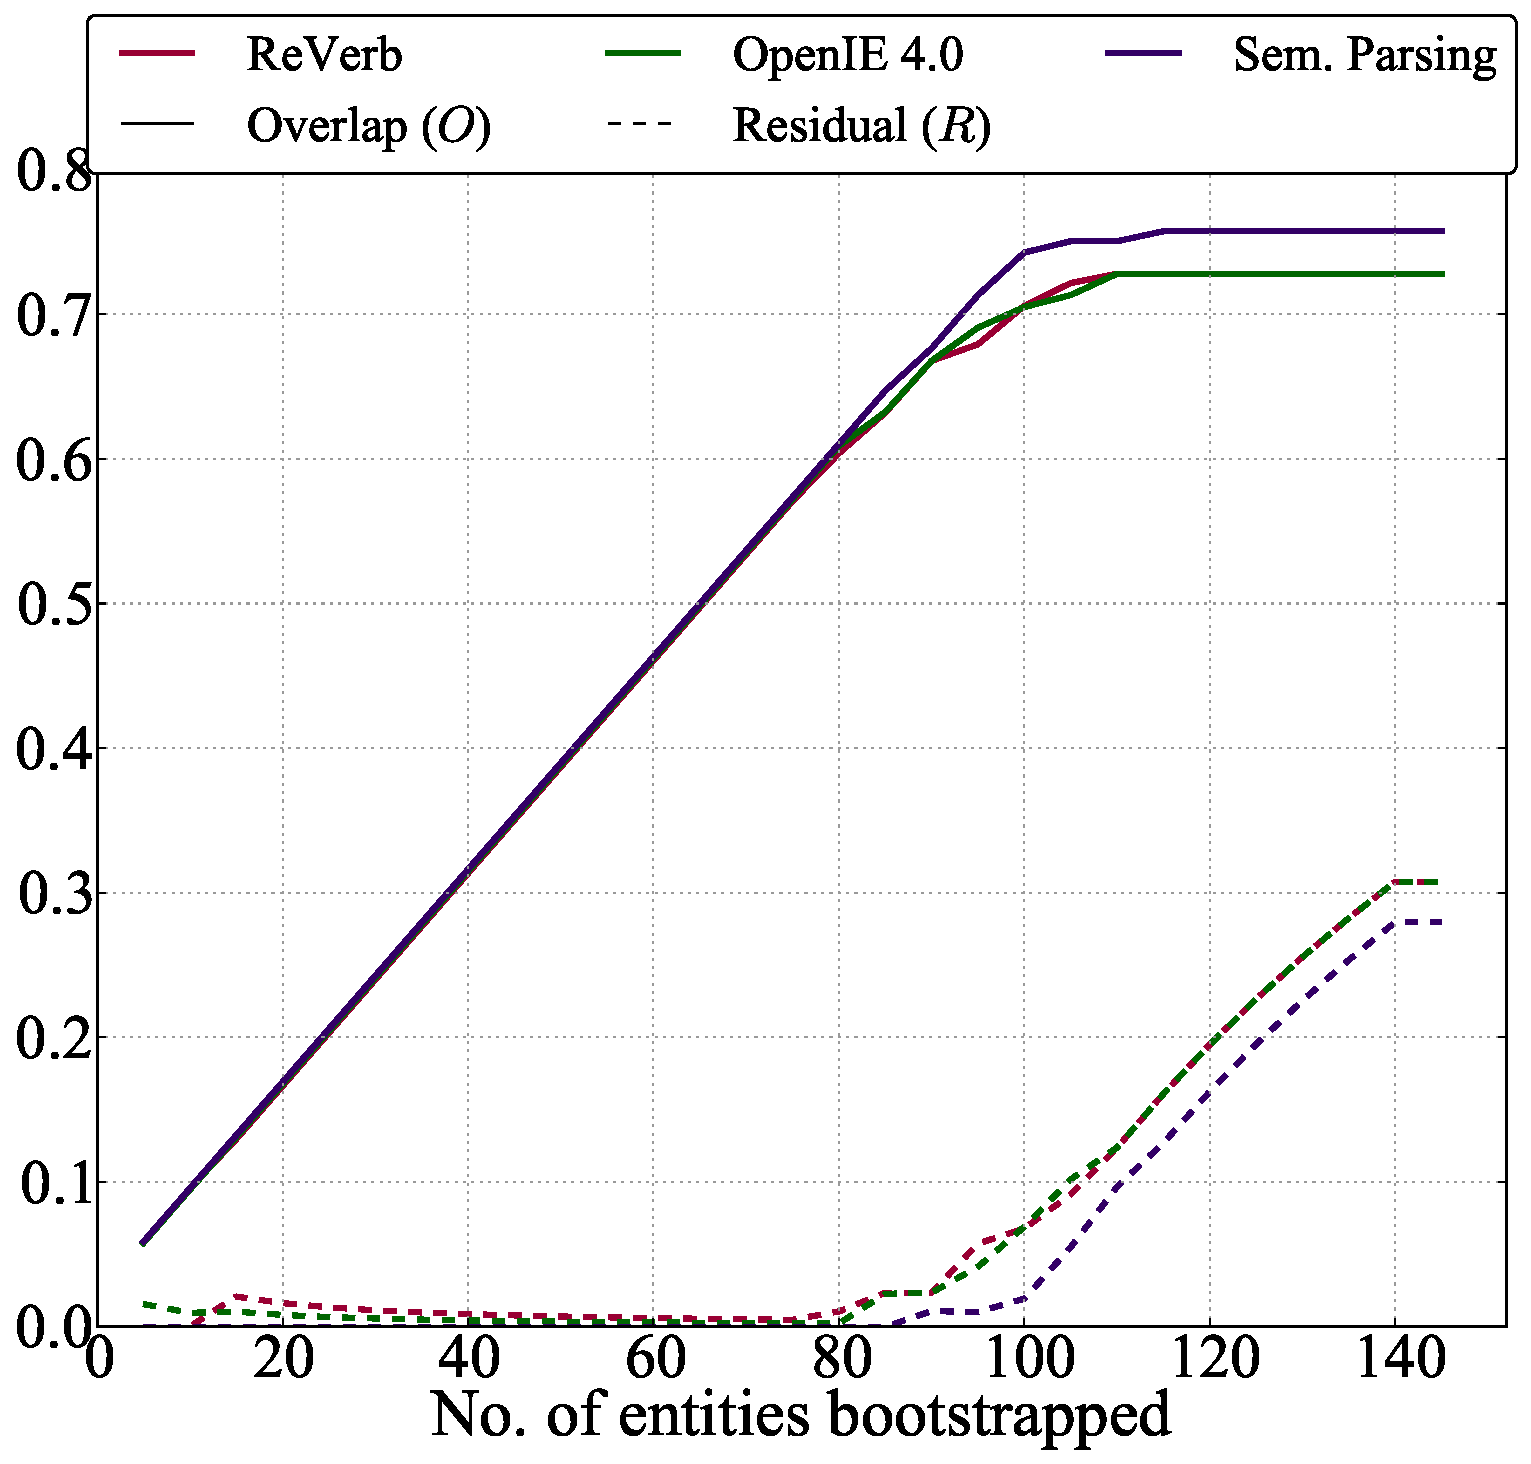
\includegraphics[width=0.45\linewidth]{../../data/results/qualitative/entity-identification/bootstrapping/carnatic_music/carnatic_ragas.pdf}
		 \label{fig:qual-object-bootstrapping-carnatic-ragas}
        }% 
        \qquad
        \subfigure[][Compositions]{%
		 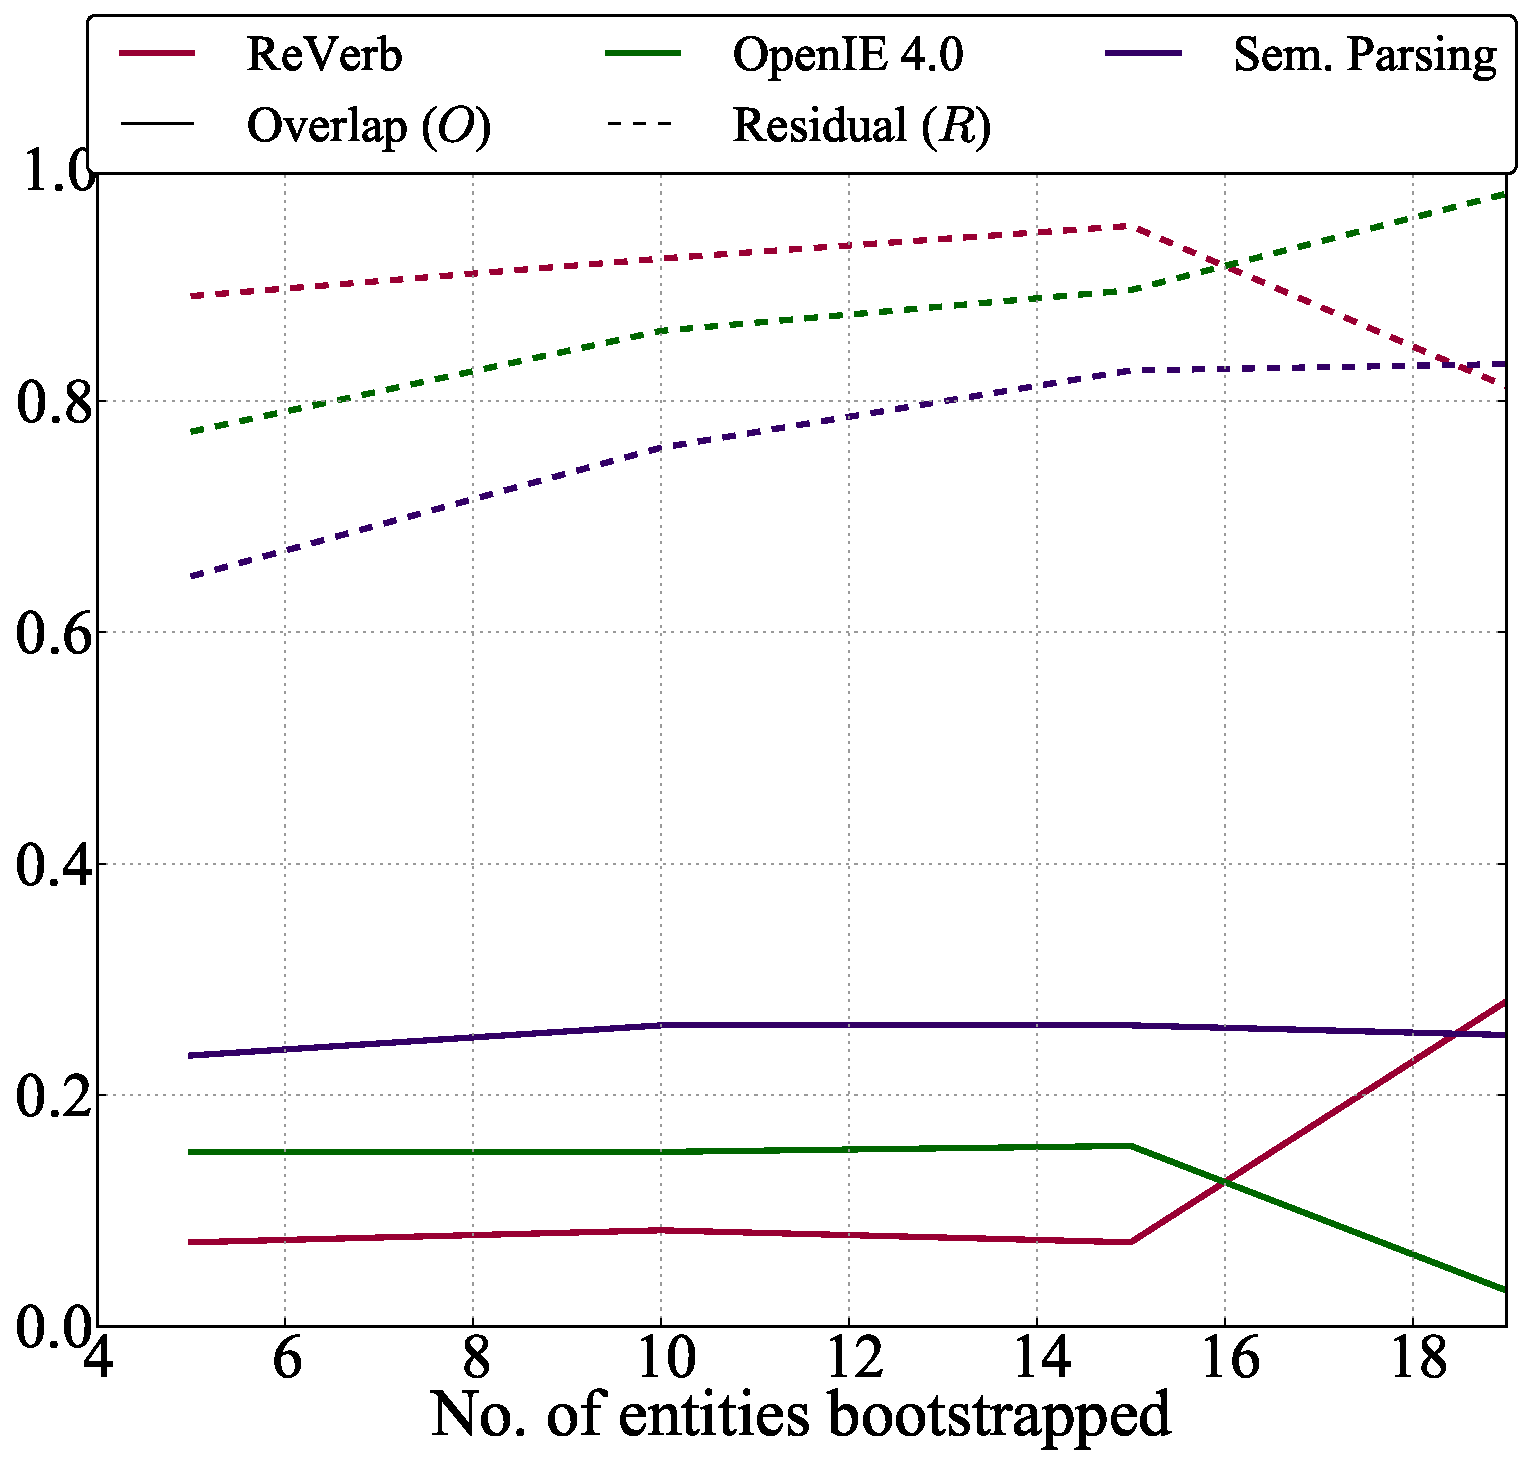
\includegraphics[width=0.45\linewidth]{../../data/results/qualitative/entity-identification/bootstrapping/carnatic_music/carnatic_compositions.pdf}
		 \label{fig:qual-object-bootstrapping-carnatic-compositions}
        }%
\end{center}
\caption{Results for bootstrapping-based concept assignment of entities identified in Carnatic music}
\label{fig:qual-object-bootstrapping-carnatic}
\end{figure}
\clearpage
}
\afterpage{
\begin{figure}[t]
\begin{center}
        \subfigure[][Musicians]{%
		 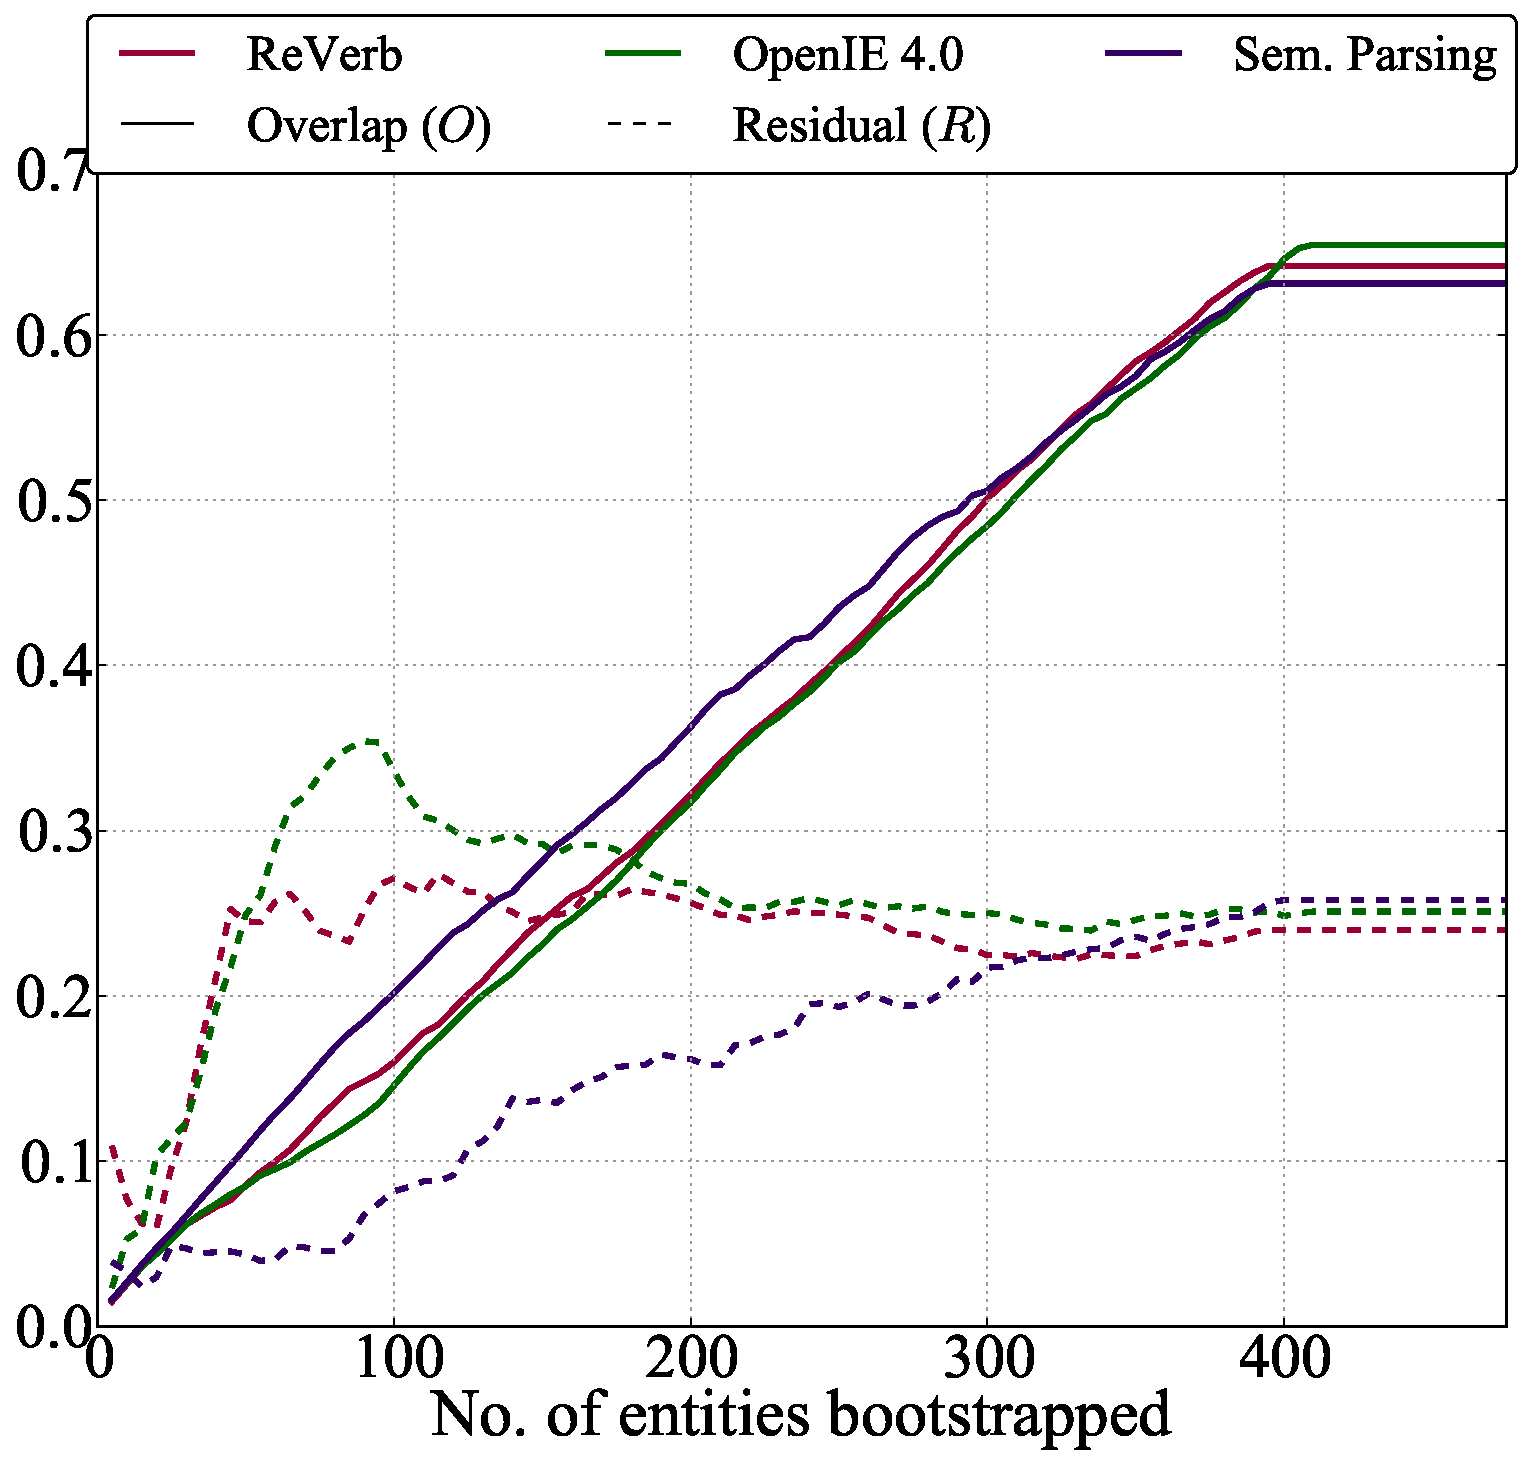
\includegraphics[width=0.45\linewidth]{../../data/results/qualitative/entity-identification/bootstrapping/hindustani_music/hindustani_musicians.pdf}
		 \label{fig:qual-object-bootstrapping-hindustani-musicians}
        }% 
        \qquad
        \subfigure[][Ragas]{%
		 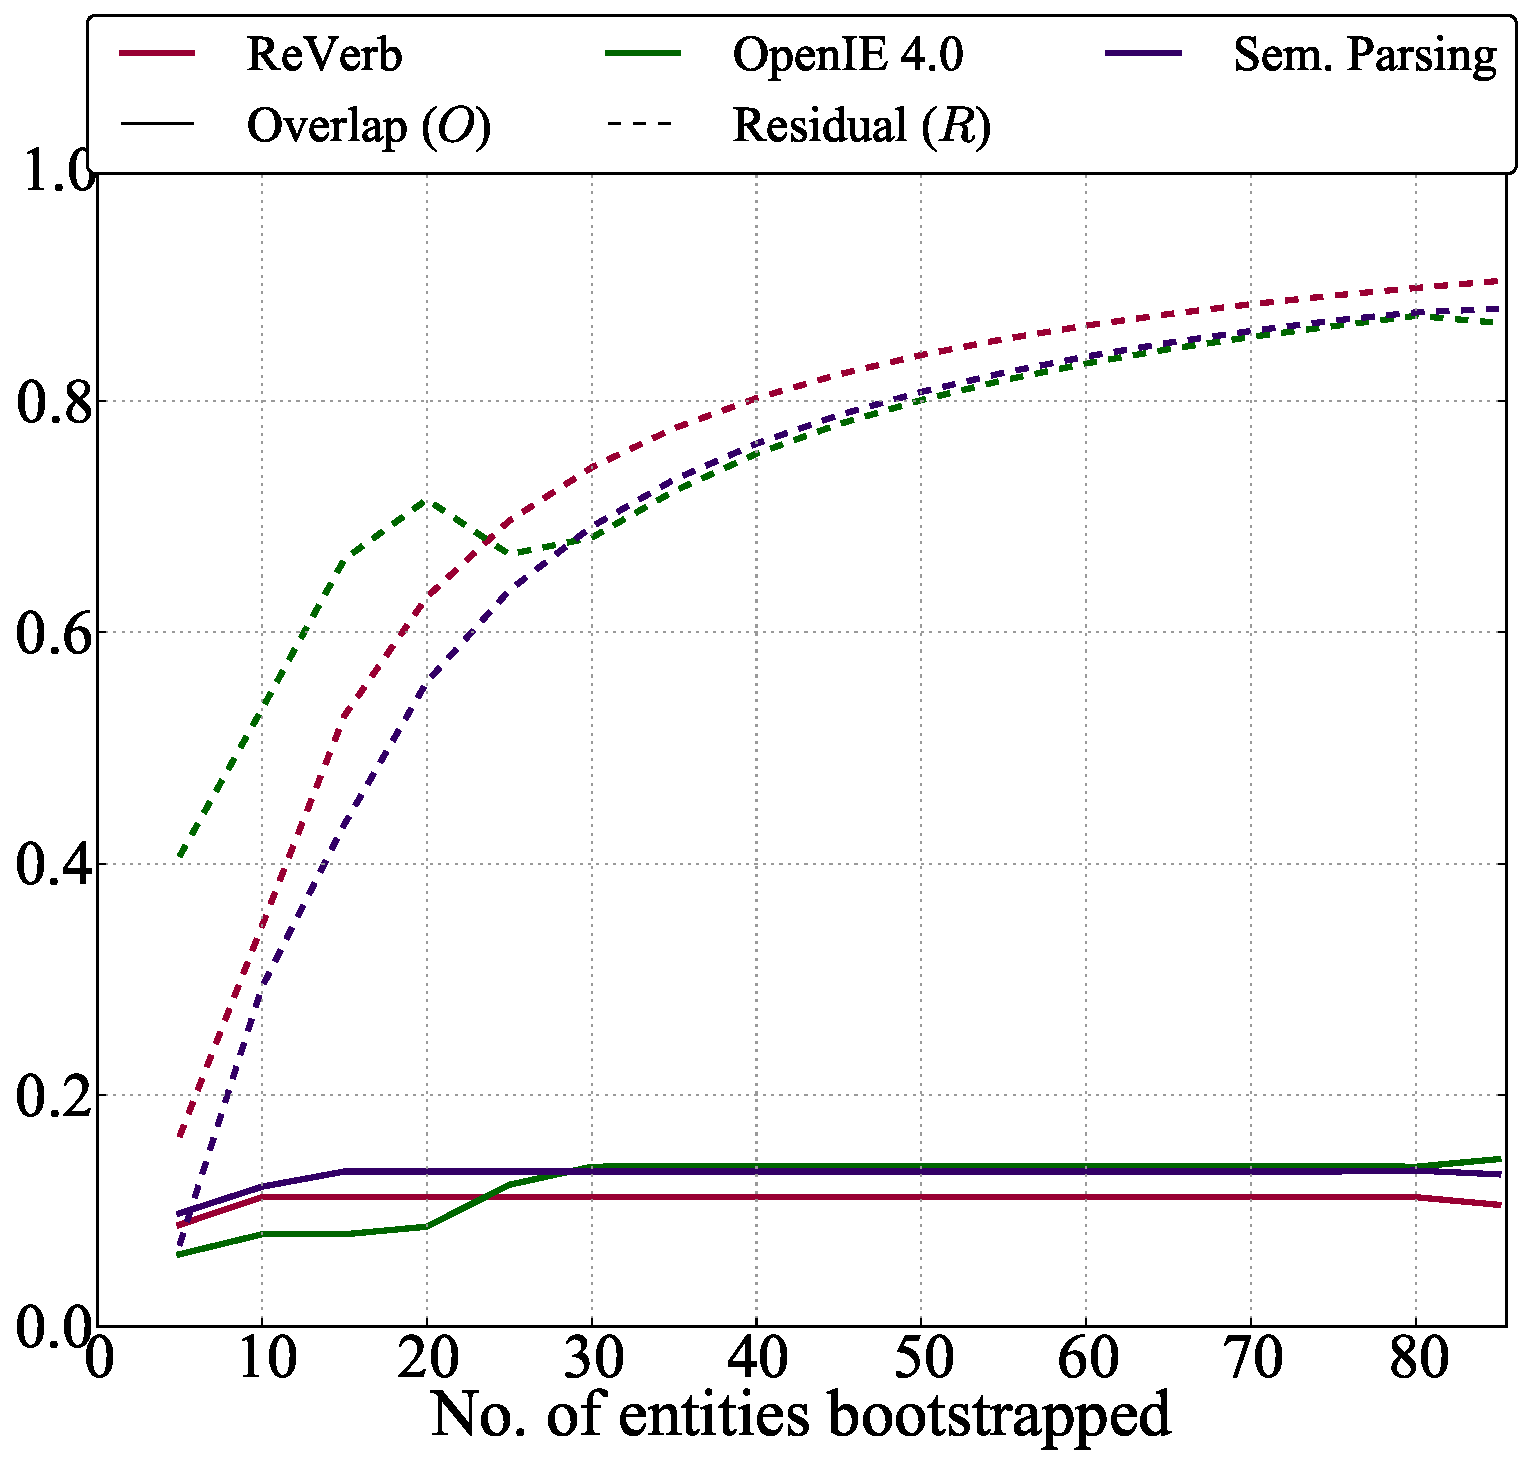
\includegraphics[width=0.45\linewidth]{../../data/results/qualitative/entity-identification/bootstrapping/hindustani_music/hindustani_ragas.pdf}
		 \label{fig:qual-object-bootstrapping-hindustani-ragas}
        }% 
%        \subfigure[][Composers]{%
%		 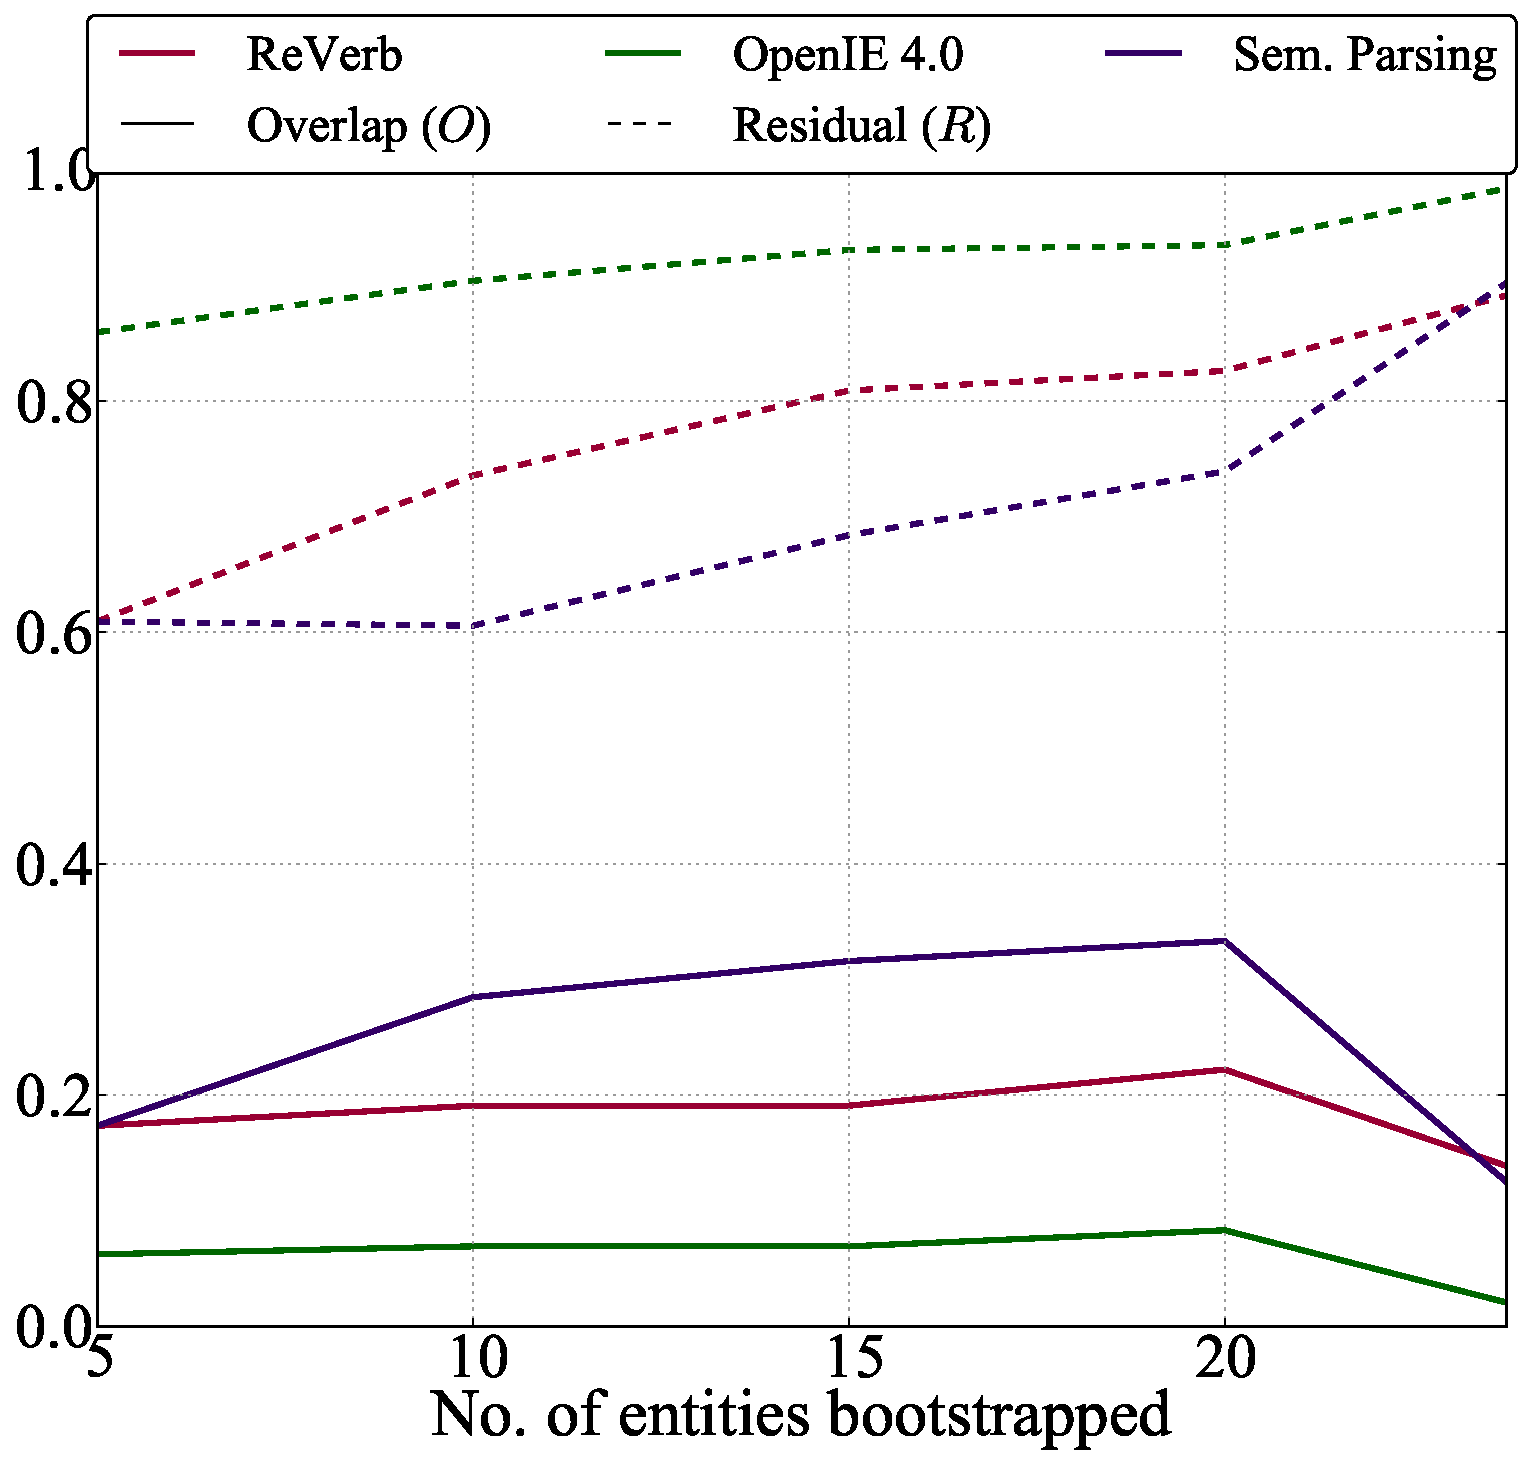
\includegraphics[width=0.45\linewidth]{../../data/results/qualitative/entity-identification/bootstrapping/hindustani_music/hindustani_composers.pdf}
%		 \label{fig:qual-object-bootstrapping-hindustani-composers}
%        }%
        \\
        \subfigure[][Instrumentalists]{%
		 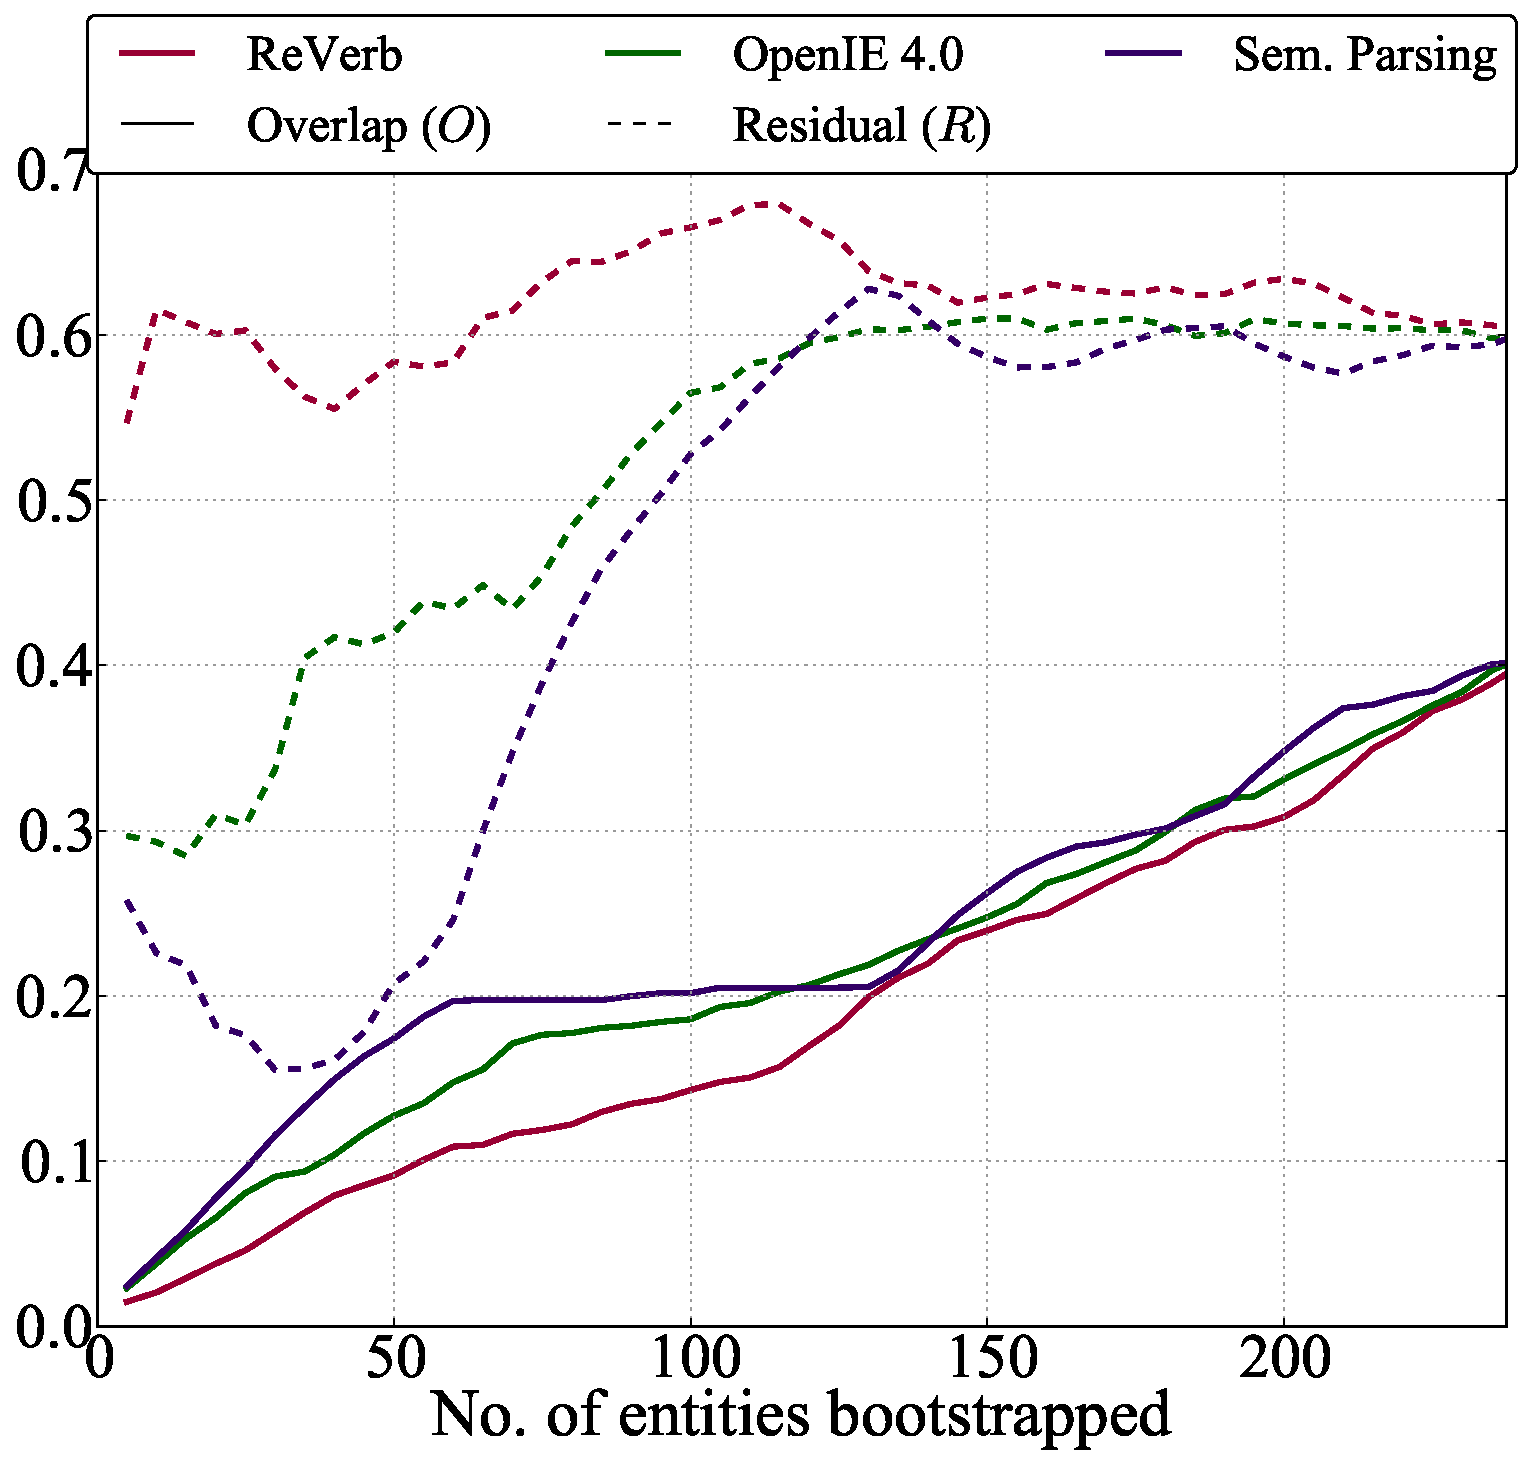
\includegraphics[width=0.45\linewidth]{../../data/results/qualitative/entity-identification/bootstrapping/hindustani_music/hindustani_instrumentalists.pdf}
		 \label{fig:qual-object-bootstrapping-hindustani-instrumentalists}
        }% 
        \qquad
        \subfigure[][Singers]{%
		 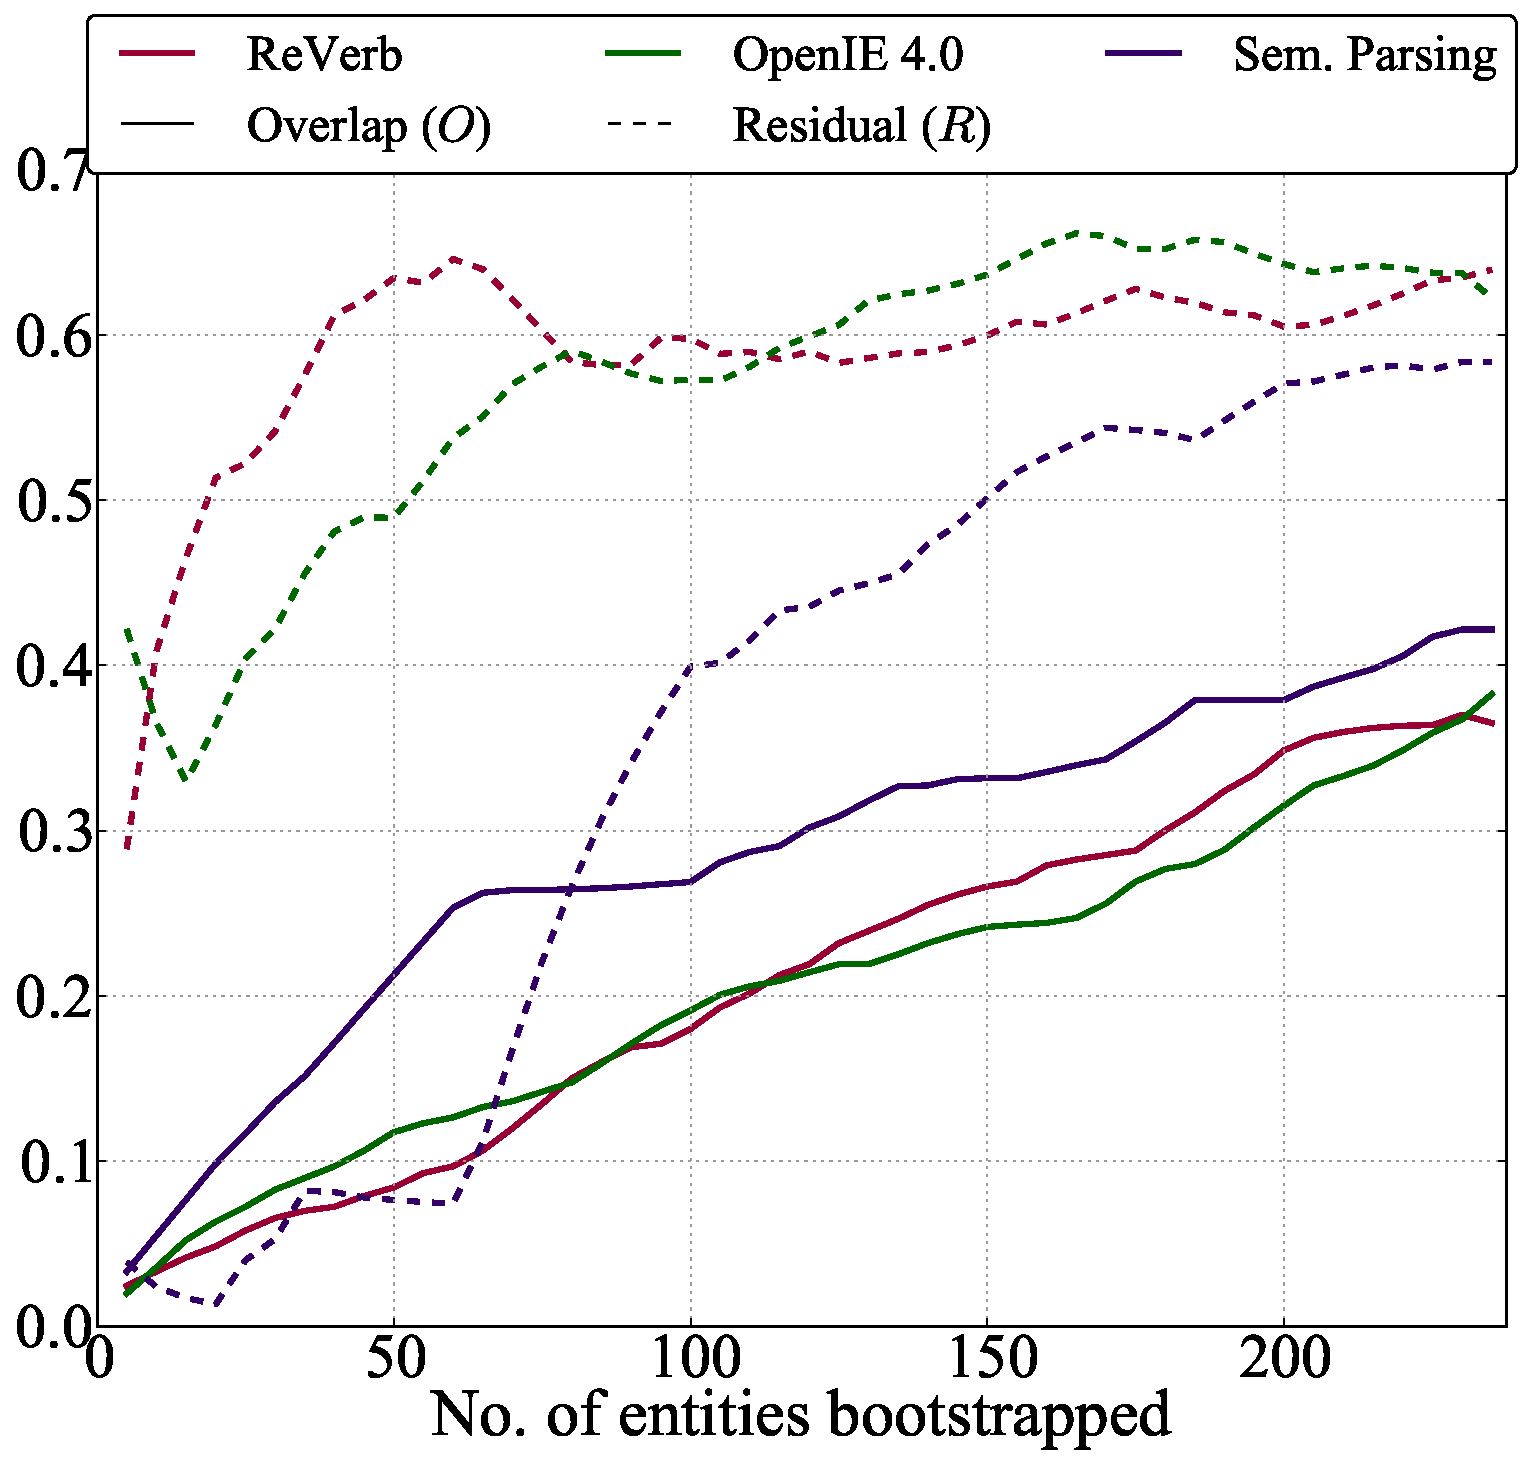
\includegraphics[width=0.45\linewidth]{../../data/results/qualitative/entity-identification/bootstrapping/hindustani_music/hindustani_singers.pdf}
		 \label{fig:qual-object-bootstrapping-hindustani-singers}
        }%
%        \\
\end{center}
\caption{Results for bootstrapping-based concept assignment of entities identified in Hindustani music. The results for hindustani composers were not included due to space constraints.}
\label{fig:qual-object-bootstrapping-hindustani}
\end{figure}
%\clearpage
}

It is noteworthy to observe that residual entity candidates are consistently less in number for the semantic parsing based system. There are two possibilities with them: they can be either false positives, or true positives which are not found in the reference data. In most cases, they are observed to be false positives. However, there are also a few of the latter. In order to understand them further, we have plotted the inter-system agreement in figs.~\ref{fig:qual-object-rulebased-carnatic-inter} and \ref{fig:qual-object-rulebased-hindustani-inter}, which is given by the cosine similarity between $R$ of different systems. ReVerb and OpenIE 4.0 agree with each other consistently higher over many of the concepts. We have observed that the cases where two or more systems agree on the candidature of a given entity, it is highly probable that the entity actually belongs to the concept. All the figures also show absolute numbers to put into perspective the proportion of residual entities where the systems agree with each other.

The second method for the evaluation of concept assignment employs bootstrapping as discussed in sec.~\ref{sec:framework}. This process involves selection of a seedset and determining the number of bootstrapping iterations. For the sake of brevity, we have set the size of seedset to be the same for all the concepts, which is 3. The entities in the seedset are randomly chosen from the ones among the reference data taken from Wikipedia. However, as the bootstrapping process itself can be sensitive to the initial selection of the entities in the seedset, the whole process is repeated 5 times with randomly chosen seedsets. The bootstrapping method is terminated once the size of seedset reaches that of the corresponding concept in the reference data. After every 5 instances added during the process, we measure the overlap ($O$) and residual ($R$) portions of the seedset with respect to the reference data.  Figs.~\ref{fig:qual-object-bootstrapping-carnatic} and \ref{fig:qual-object-bootstrapping-hindustani} show their mean over 5 runs. 
\afterpage{
\begin{figure}[!t]
\begin{center}
        \subfigure[][Carnatic music: No. of valid relation types]{%
		 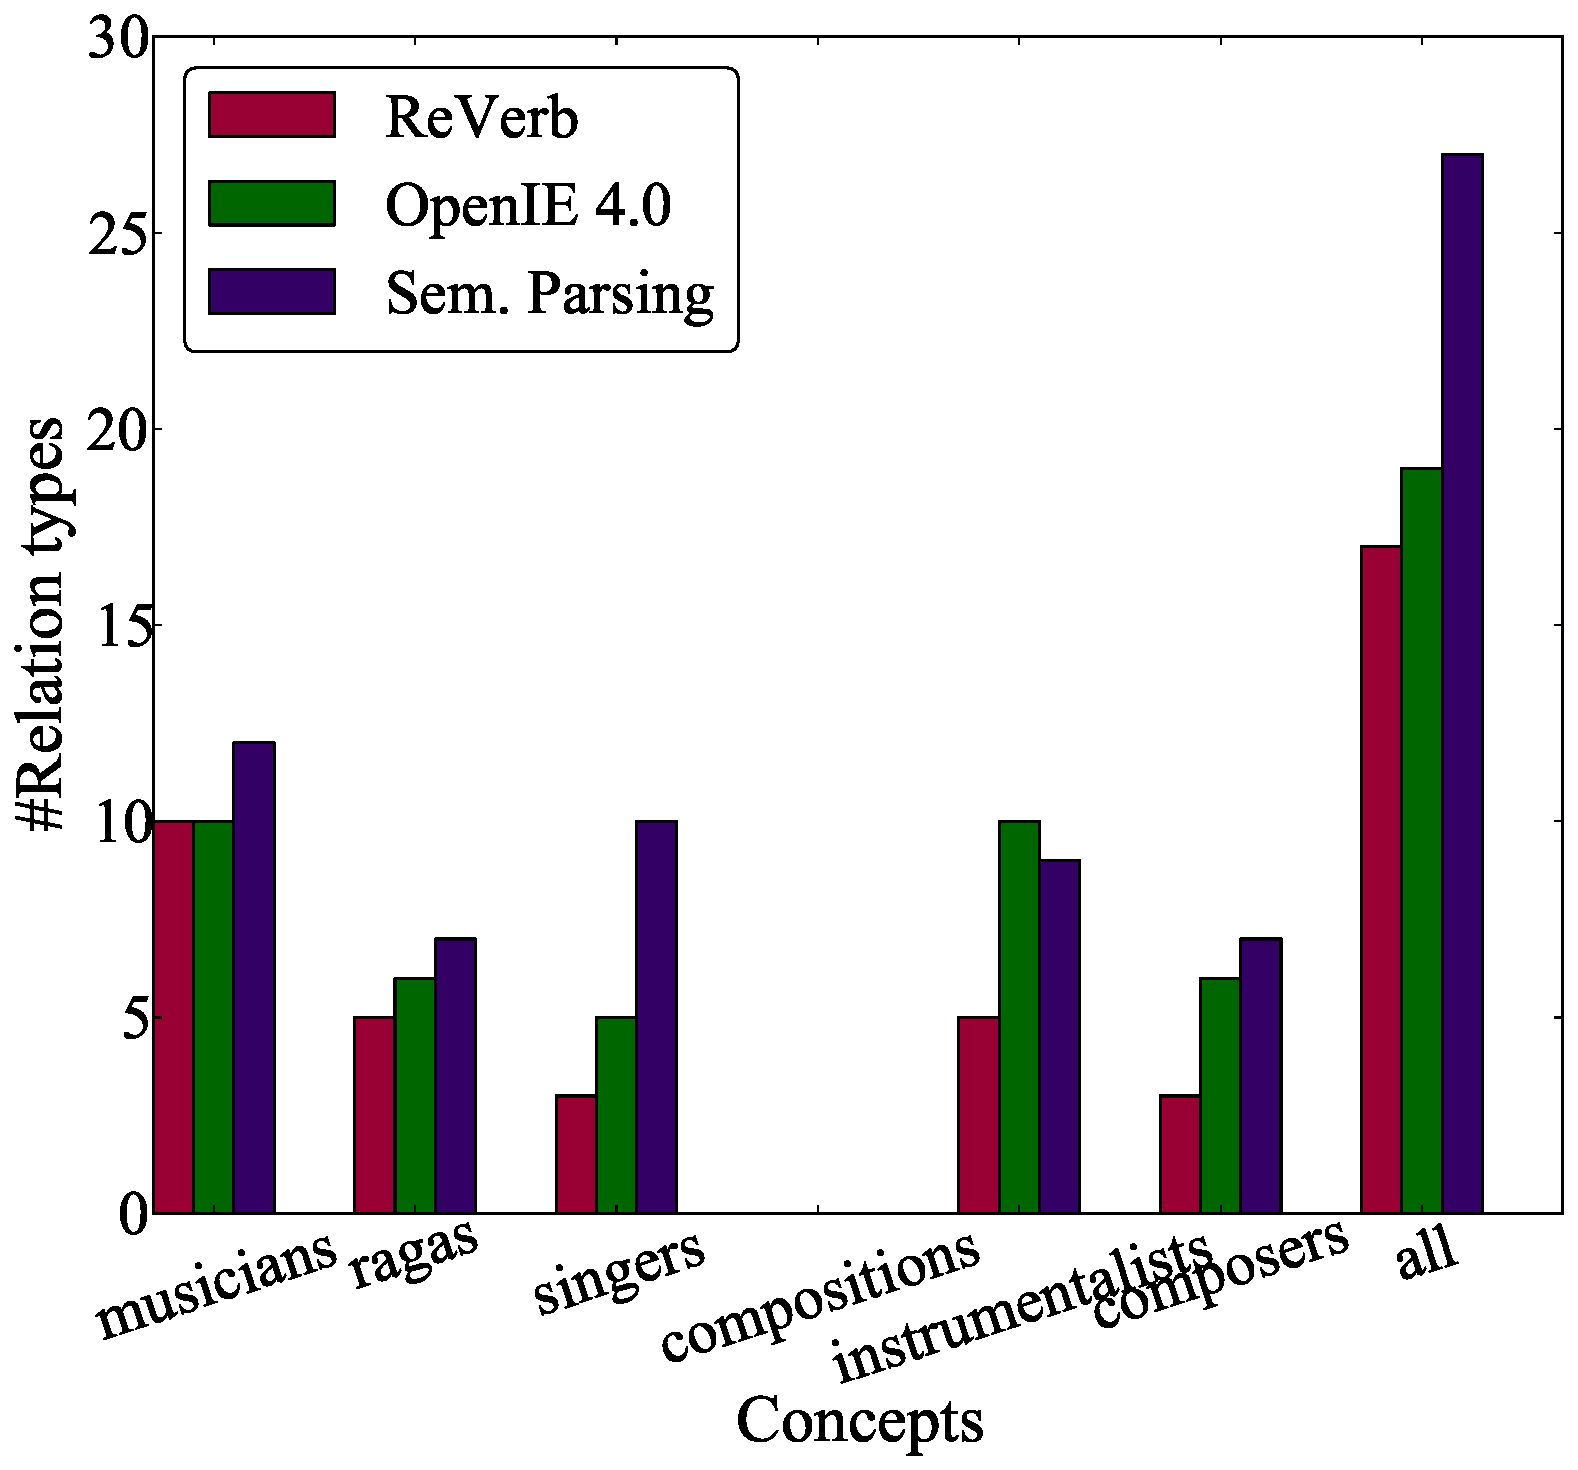
\includegraphics[width=0.45\linewidth]{../../data/results/qualitative/semantic-relation-extraction/carnatic_music.pdf}
		 \label{fig:qual-semantic-relex-carnatic}
        }% 
        \qquad
        \subfigure[][Carnatic music: No. of corresponding assertions]{%
		 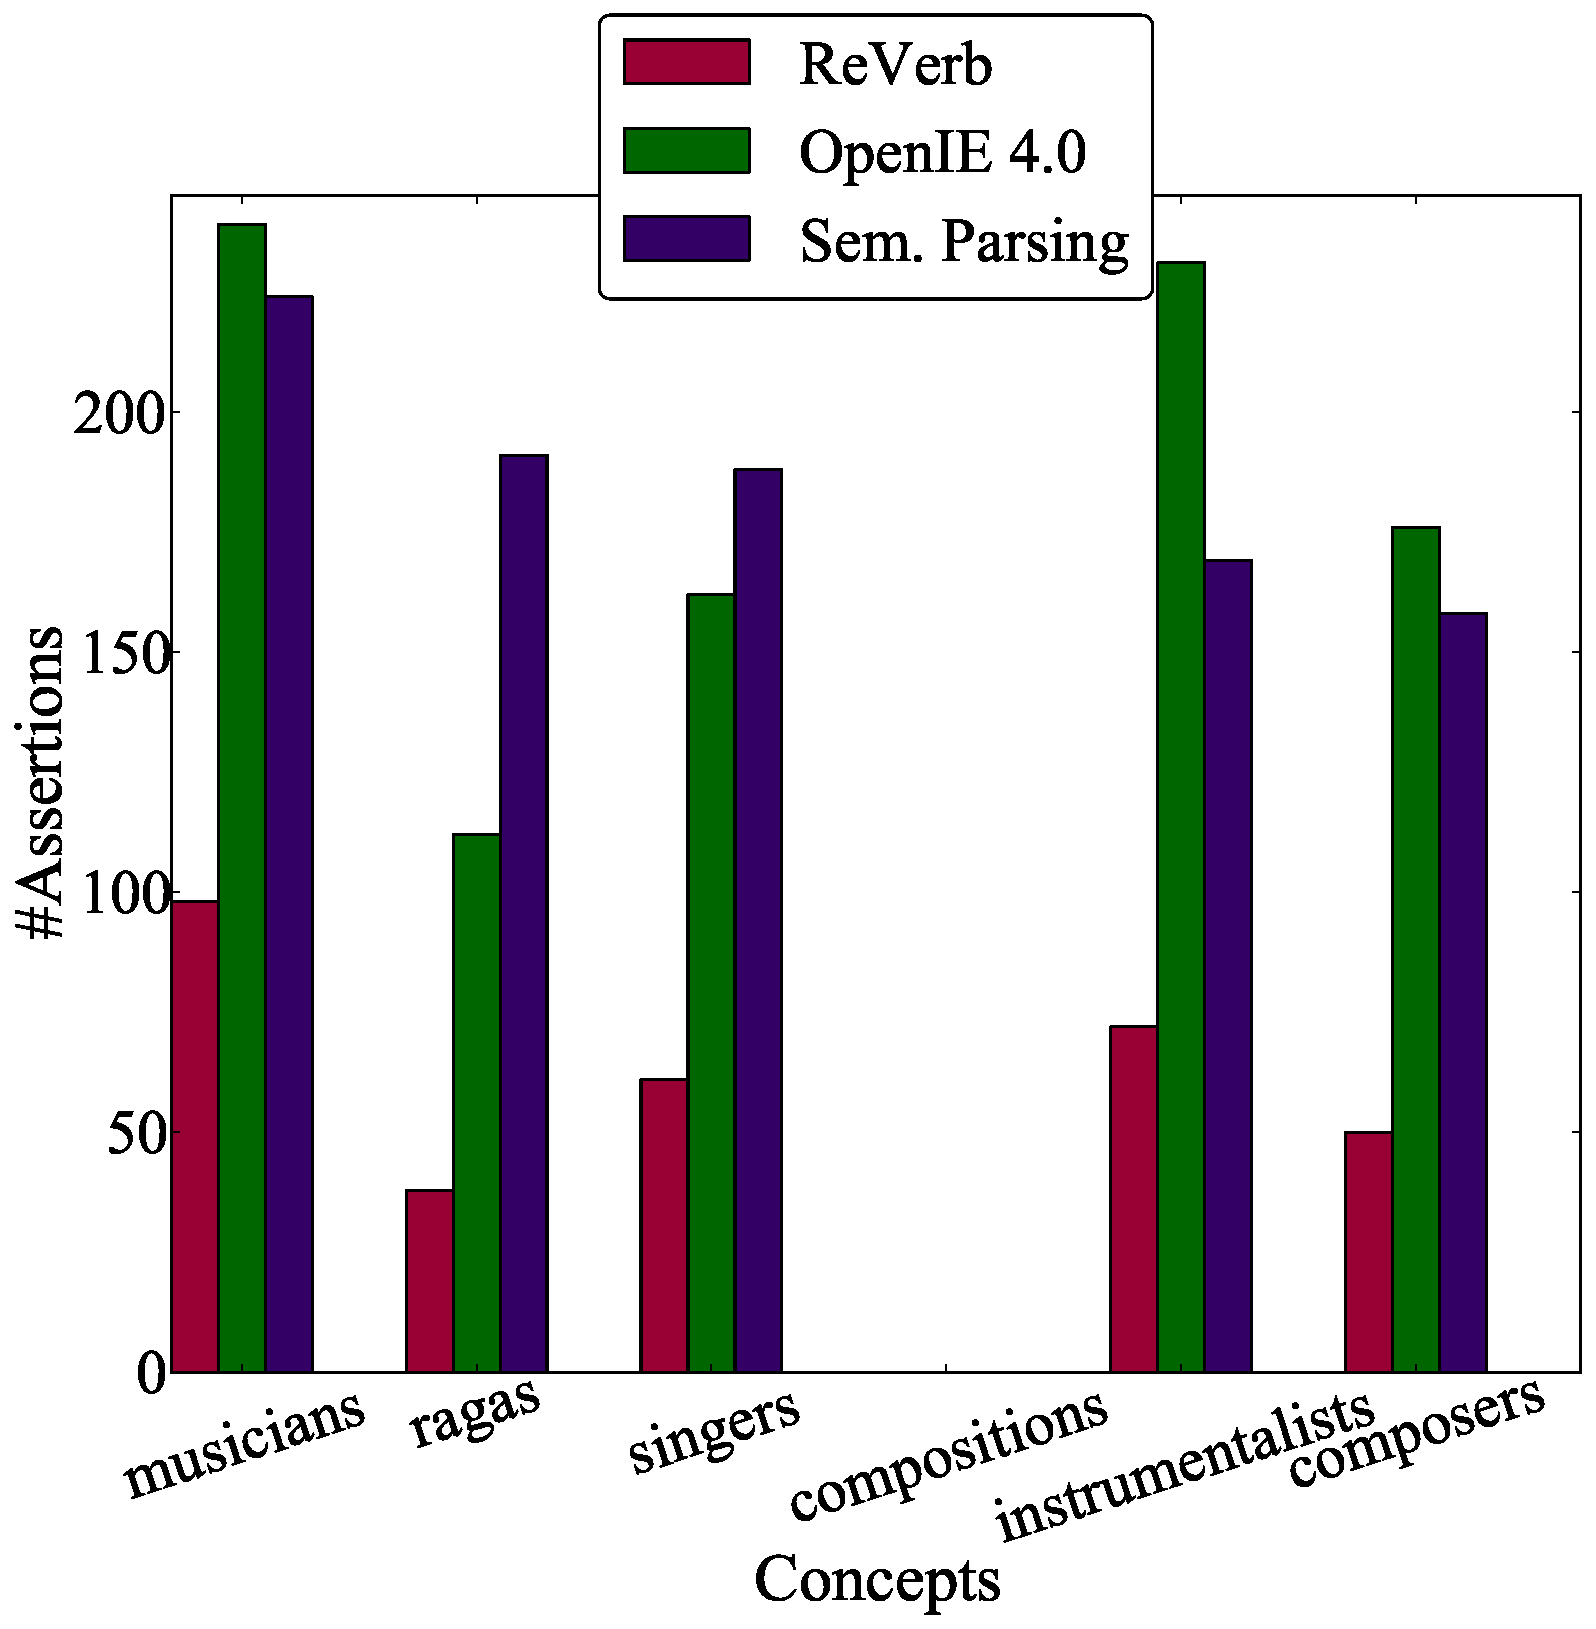
\includegraphics[width=0.45\linewidth]{../../data/results/qualitative/semantic-relation-extraction/carnatic_music-relcount.pdf}
		 \label{fig:qual-semantic-relex-carnatic-relcount}
        }%
        \\
        \subfigure[][Hindustani music: No. of valid relation types]{%
		 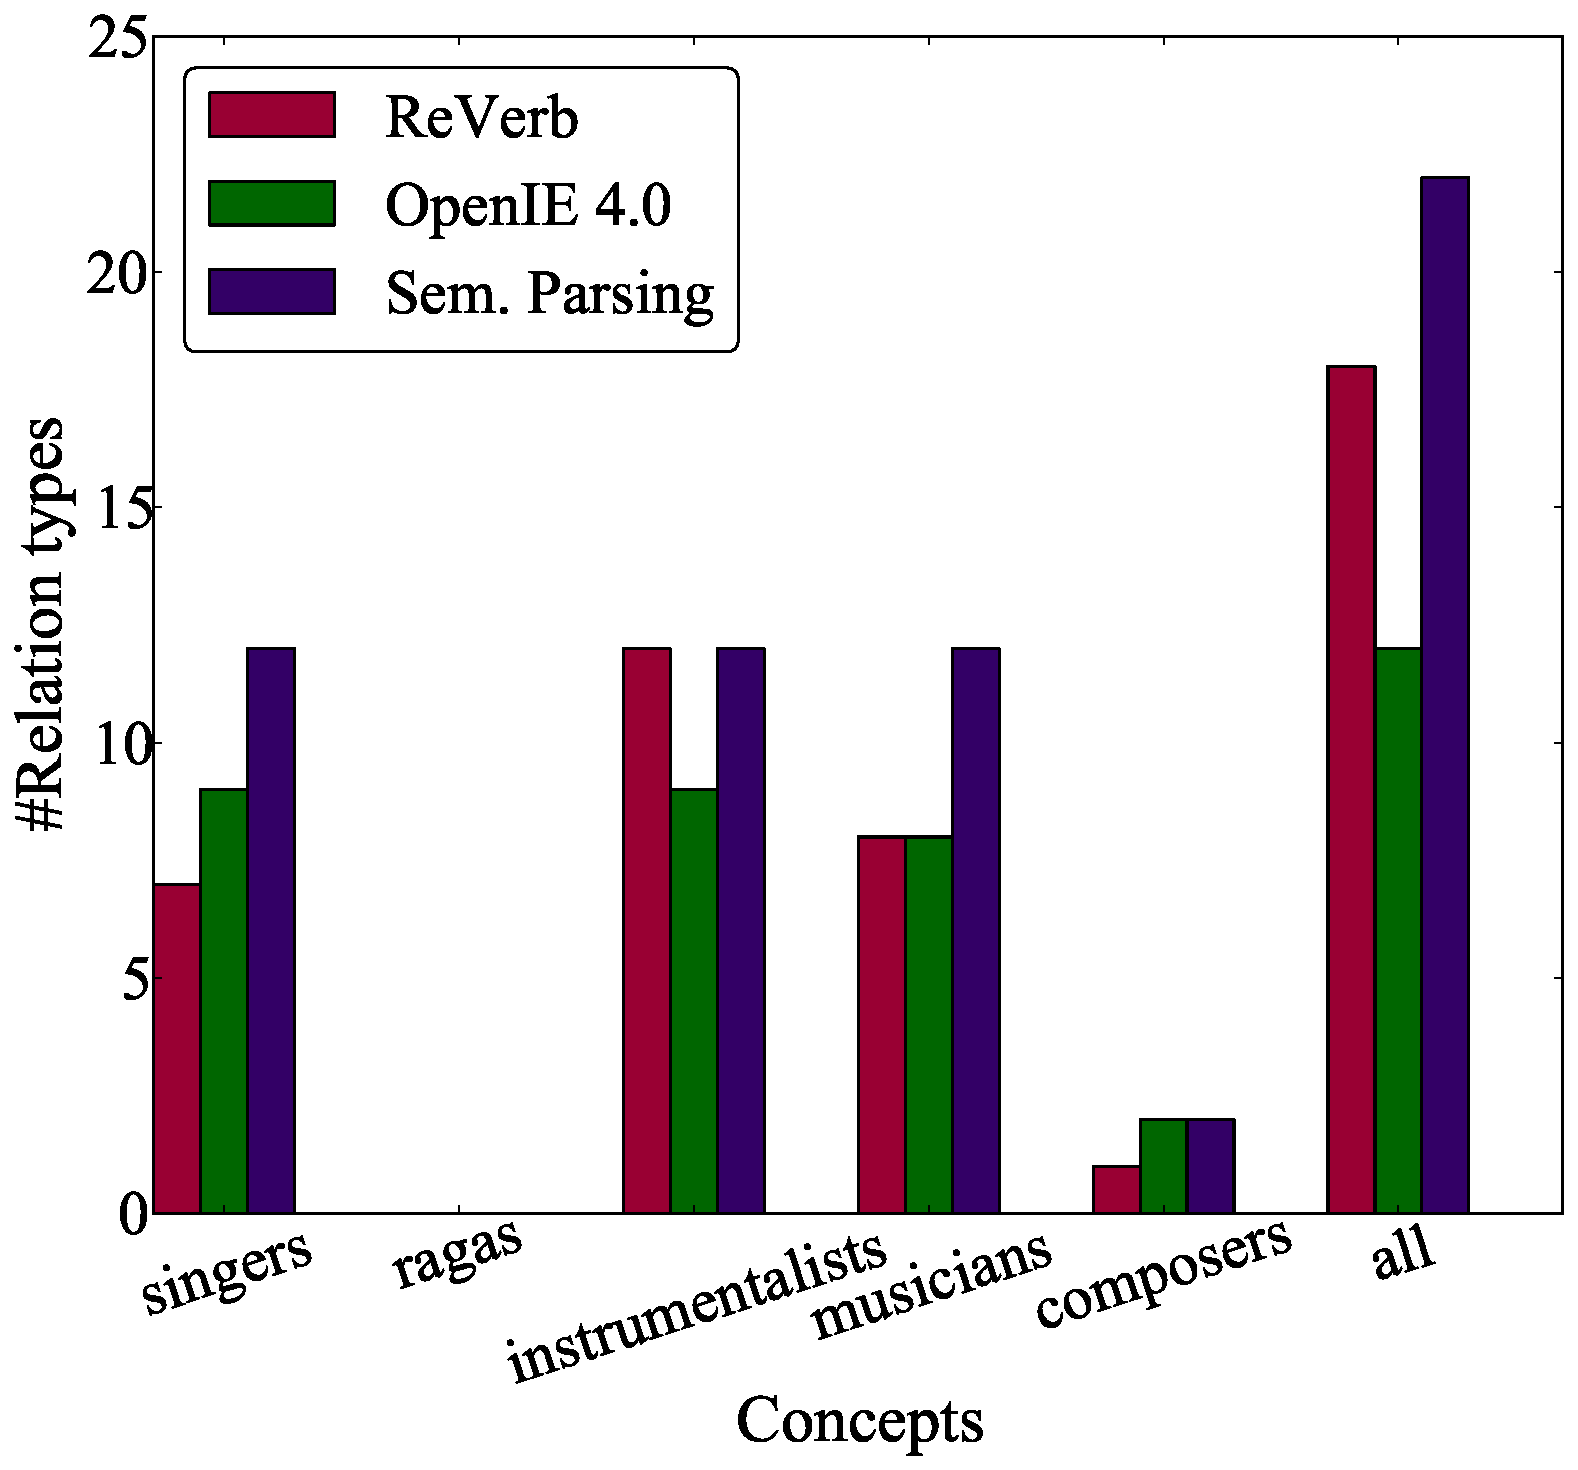
\includegraphics[width=0.45\linewidth]{../../data/results/qualitative/semantic-relation-extraction/hindustani_music.pdf}
		 \label{fig:qual-semantic-relex-hindustani}
        }%
        \qquad
        \subfigure[][Hindustani music: No. of corresponding assertions]{%
		 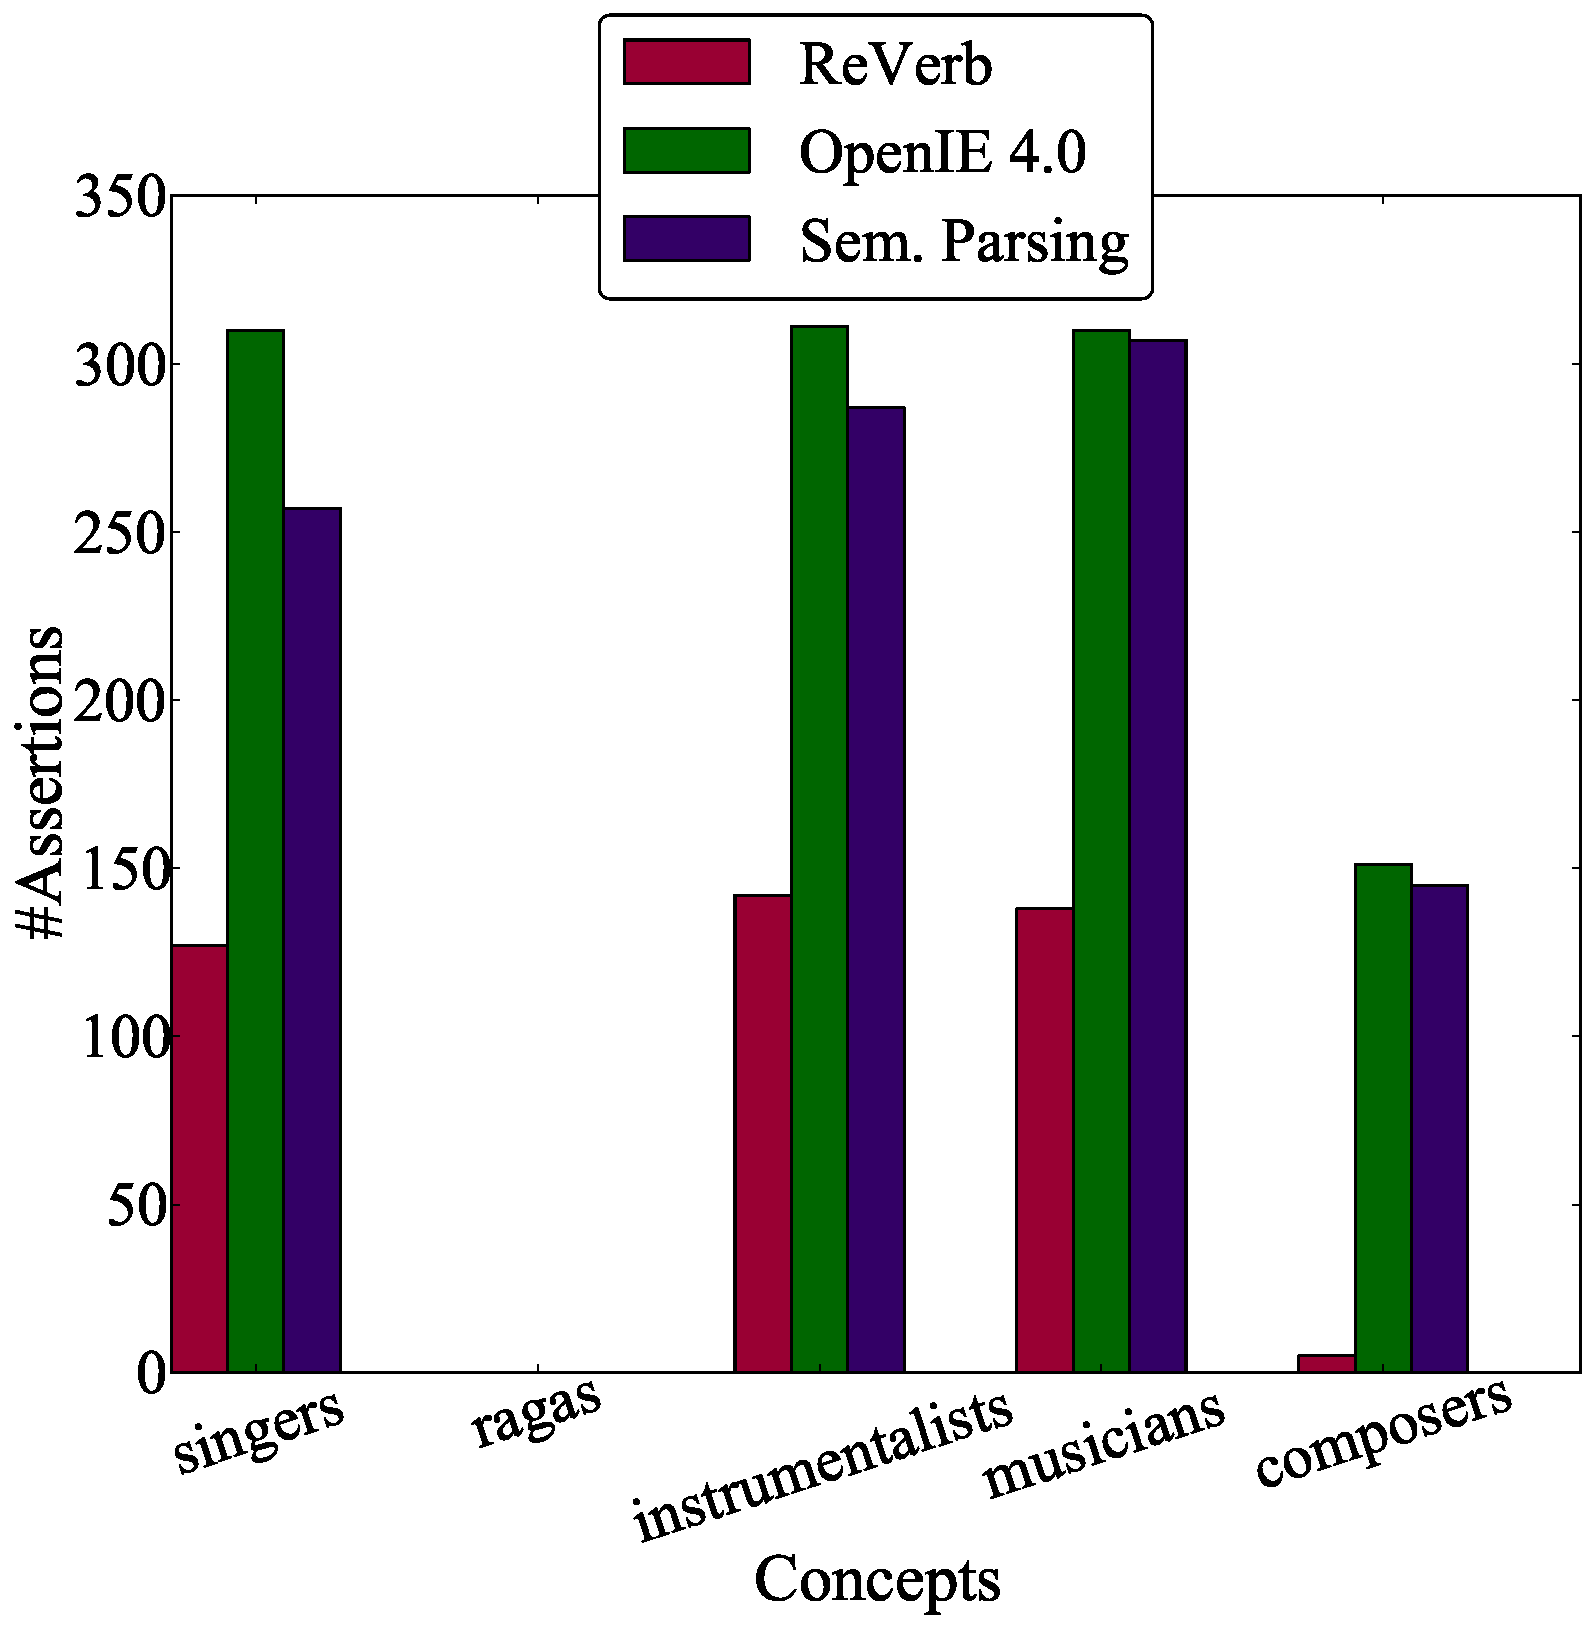
\includegraphics[width=0.45\linewidth]{../../data/results/qualitative/semantic-relation-extraction/hindustani_music-relcount.pdf}
		 \label{fig:qual-semantic-relex-hindustani-relcount}
        }%
\end{center}
\caption{Semantic relation extraction task: The number of valid relation types marked for each concept, and the number of corresponding assertions that include the entities in the domain.}
\label{fig:qual-semantic-relex}
\end{figure}
}

In most categories and for all the three systems, it can be seen that $R$ grows quickly over iterations, making the residual portion the majority among the candidate entities, which brings the precision down. The semantic parsing based system consistently outperforms the other two methods, both in terms of having higher $O$, and lower $R$. Between ReVerb and OpenIE 4.0, there is no substantial difference in terms of $O$. For Carnatic singer and instrumentalist categories, however, the latter results in a lower $R$, and a slightly higher $O$ compared to the former. These results partly contrast with those obtained for the rule-based concept assignment (fig.~\ref{fig:qual-object-rulebased}). However, remember that the coverage of concepts in the domain is observed to be remarkably better in the case of the semantic parsing based system 
(figs.~\ref{fig:quant-carnatic-concept} and~\ref{fig:quant-hindustani-concept}). As the bootstrapping method uses the objects from the triples (which are the candidate concepts), it seems logical that the semantic parsing based system has performed substantially better than the other two.

\paragraph{Semantic relation extraction.}
For the purpose of this task, the subsumption relation types and also those relation phrases which do not have a consistent meaning across the assertions were discarded. Then, following the procedure discussed in sec.\ref{sec:framework}, we have marked the valid relation types for each concept, and obtained the corresponding assertions featuring the entities in the domain. Fig.~\ref{fig:qual-semantic-relex} shows the results, for both Carnatic and Hindustani music. 

In terms of the breadth of the valid relation types (see sec.~\ref{sec:framework}), the semantic parsing based system performs better than OpenIE 4.0, which in most cases fares better than ReVerb. However, in terms of the depth of relation types, both the semantic parsing based system and OpenIE 4.0 perform competitively, with the former scoring high in a few categories while the latter in few others. Compared to these two, ReVerb scores substantially less in this task. This can be attributed to two reasons: the former two handle noun-mediated relations, whereas ReVerb does not, the average number of assertions for a noun-mediated relation type is observed to be usually higher than the verb-mediated relations. The second reason can be specific to the domain, where the relations with musical concepts are mostly noun-mediated (e.g: Abhogi, is a raga in, Carnatic music). Notice that there is a strong concurrence between these results and those shown in figs.~\ref{fig:quant-carnatic-reltype} and \ref{fig:quant-hindustani-reltype}, with a noticeable correlation in the differences between the performance of the OIE systems.

\section{Conclusions and Future work}
\label{sec:conclusions}
In this paper, we have presented a framework for comparative evaluation of open information extraction systems for ontologization of thematic domains. We have demonstrated it using three OIE systems in ontologizing the Indian art music domain. The results lead us to better understand the behavior of the systems from different perspectives, which can be used to guide the future research in adapting OIE to thematic domains. The source code for the framework, links to various software components used in the demonstration, the ontologies and the data are made available online\footnote{https://github.com/gopalkoduri/openie\_eval\\Documentation and code streamlining are underway.}. 

A particular limitation of the framework that is of concern is the availability of groudtruth for qualitative evaluation. The current framework hinges on to the structured content in Wikipedia/DBpedia to this extent. However, as our case study with Indian art music shows, they lack finer segregation of concepts (refer to the ontologies linked with this paper). As we have seen, the results from the quantitative and the qualitative evaluation have a strong agreement with each other. We would like to further explore this correlation using other domains, in order to better understand it and adapt the framework to meet this challenge.

\paragraph{\textbf{Acknowledgments.}} This research was partly funded by the European Research Council under the European Union's Seventh Framework Program, as part of the CompMusic project (ERC grant agreement 267583).

\renewcommand\bibname{References}
{\fontsize{9}{10}\selectfont
\footnotesize
\bibliography{references}
\bibliographystyle{splncs}
}
\end{document}
